% A LaTeX template for MSc Thesis submissions to 
% Politecnico di Milano (PoliMi) - School of Industrial and Information Engineering
%
% https://www.ingindinf.polimi.it/it/didattica/lezioni-e-esami/esami-di-laurea-e-laurea-magistrale
%
% S. Bonetti, A. Gruttadauria, G. Mescolini, A. Zingaro
% e-mail: template-tesi-ingind@polimi.it
%
% Last Revision: October 2021
%
% Copyright 2021 Politecnico di Milano, Italy. NC-BY

\documentclass{Configuration_Files/PoliMi3i_thesis}

%------------------------------------------------------------------------------
%	REQUIRED PACKAGES AND  CONFIGURATIONS
%------------------------------------------------------------------------------

% CONFIGURATIONS
\usepackage{parskip} % For paragraph layout
\usepackage{setspace} % For using single or double spacing
\usepackage{emptypage} % To insert empty pages
\usepackage{multicol} % To write in multiple columns (executive summary)
\setlength\columnsep{15pt} % Column separation in executive summary
\setlength\parindent{0pt} % Indentation
\raggedbottom  

% PACKAGES FOR TITLES
\usepackage{titlesec}
% \titlespacing{\section}{left spacing}{before spacing}{after spacing}
\titlespacing{\section}{0pt}{3.3ex}{2ex}
\titlespacing{\subsection}{0pt}{3.3ex}{1.65ex}
\titlespacing{\subsubsection}{0pt}{3.3ex}{1ex}
\usepackage{color}

% PACKAGES FOR LANGUAGE AND FONT
\usepackage[english]{babel} % The document is in English  
\usepackage[utf8]{inputenc} % UTF8 encoding
\usepackage[T1]{fontenc} % Font encoding
\usepackage[11pt]{moresize} % Big fonts

% PACKAGES FOR IMAGES
\usepackage{graphicx}
\usepackage{transparent} % Enables transparent images
\usepackage{eso-pic} % For the background picture on the title page
\usepackage{subfig} % Numbered and caption subfigures using \subfloat.
\usepackage{tikz} % A package for high-quality hand-made figures.
\usetikzlibrary{}
\graphicspath{{./Images/}} % Directory of the images
\usepackage{caption} % Coloured captions
\usepackage{xcolor} % Coloured captions
\usepackage{amsthm,thmtools,xcolor} % Coloured "Theorem"
\usepackage{float}

% STANDARD MATH PACKAGES
\usepackage{amsmath}
\usepackage{amsthm}
\usepackage{amssymb}
\usepackage{amsfonts}
\usepackage{bm}
\usepackage[overload]{empheq} % For braced-style systems of equations.
\usepackage{fix-cm} % To override original LaTeX restrictions on sizes

% PACKAGES FOR TABLES
\usepackage{tabularx}
\usepackage{longtable} % Tables that can span several pages
\usepackage{colortbl}

% PACKAGES FOR ALGORITHMS (PSEUDO-CODE)
\usepackage{algorithm}
\usepackage{algorithmic}

% PACKAGES FOR REFERENCES & BIBLIOGRAPHY
\usepackage[colorlinks=true,linkcolor=black,anchorcolor=black,citecolor=black,filecolor=black,menucolor=black,runcolor=black,urlcolor=black]{hyperref} % Adds clickable links at references
\usepackage{cleveref}
\usepackage[square, numbers, sort&compress]{natbib} % Square brackets, citing references with numbers, citations sorted by appearance in the text and compressed
\bibliographystyle{abbrvnat} % You may use a different style adapted to your field

% OTHER PACKAGES
\usepackage{pdfpages} % To include a pdf file
\usepackage{afterpage}
\usepackage{lipsum} % DUMMY PACKAGE
\usepackage{fancyhdr} % For the headers
\fancyhf{}

% Input of configuration file. Do not change config.tex file unless you really know what you are doing. 
% Set the geometric layout of the document
\usepackage{geometry}
\geometry{
  top=2.8cm,
  left = 1.9cm,
  right = 1.9cm,
  bottom=2.0cm,
  headheight= 2cm,
  headsep= 0cm,
}
\raggedbottom 

% Create color bluePoli (-> manuale grafica coordinata:  https://www.polimi.it/fileadmin/user_upload/il_Politecnico/grafica-coordinata/2015_05_11_46xy_manuale_grafica_coordinata.pdf)
\definecolor{bluePoli}{cmyk}{0.4,0.1,0,0.4}

% Custom theorem environments
\declaretheoremstyle[
  headfont=\color{bluePoli}\normalfont\bfseries,
  bodyfont=\color{black}\normalfont\itshape,
]{colored}

\captionsetup[figure]{labelfont={color=bluePoli}} % Set colour of the captions
\captionsetup[table]{labelfont={color=bluePoli}} % Set colour of the captions
\captionsetup[algorithm]{labelfont={color=bluePoli}} % Set colour of the captions

\theoremstyle{colored}
\newtheorem{theorem}{Theorem}[section]
\newtheorem{proposition}{Proposition}[section]

% Enhances the features of the standard "table" and "tabular" environments.
\newcommand\T{\rule{0pt}{2.6ex}}
\newcommand\B{\rule[-1.2ex]{0pt}{0pt}}

% Algorithm description
\newcounter{algsubstate}
\renewcommand{\thealgsubstate}{\alph{algsubstate}}
\newenvironment{algsubstates}{
    \setcounter{algsubstate}{0}%
    \renewcommand{\STATE}{%
    \stepcounter{algsubstate}%
    \Statex {\small\thealgsubstate:}\space}
    }{}
    
% Custom theorem environment
\newcolumntype{L}[1]{>{\raggedright\let\newline\\\arraybackslash\hspace{0pt}}m{#1}}
\newcolumntype{C}[1]{>{\centering\let\newline\\\arraybackslash\hspace{0pt}}m{#1}}
\newcolumntype{R}[1]{>{\raggedleft\let\newline\\\arraybackslash\hspace{0pt}}m{#1}}

% Custom itemize environment
\setlist[itemize,1]{label=$\bullet$}
\setlist[itemize,2]{label=$\circ$}
\setlist[itemize,3]{label=$-$}
\setlist{nosep}

% Set separation of columns 
\setlength{\columnsep}{30pt}

% Create command for background pic
\newcommand\BackgroundPic{% Adding background picture
	\put(237,365){
		\parbox[b][\paperheight]{\paperwidth}{%
			\vfill
			\centering
			\transparent{0.4}
			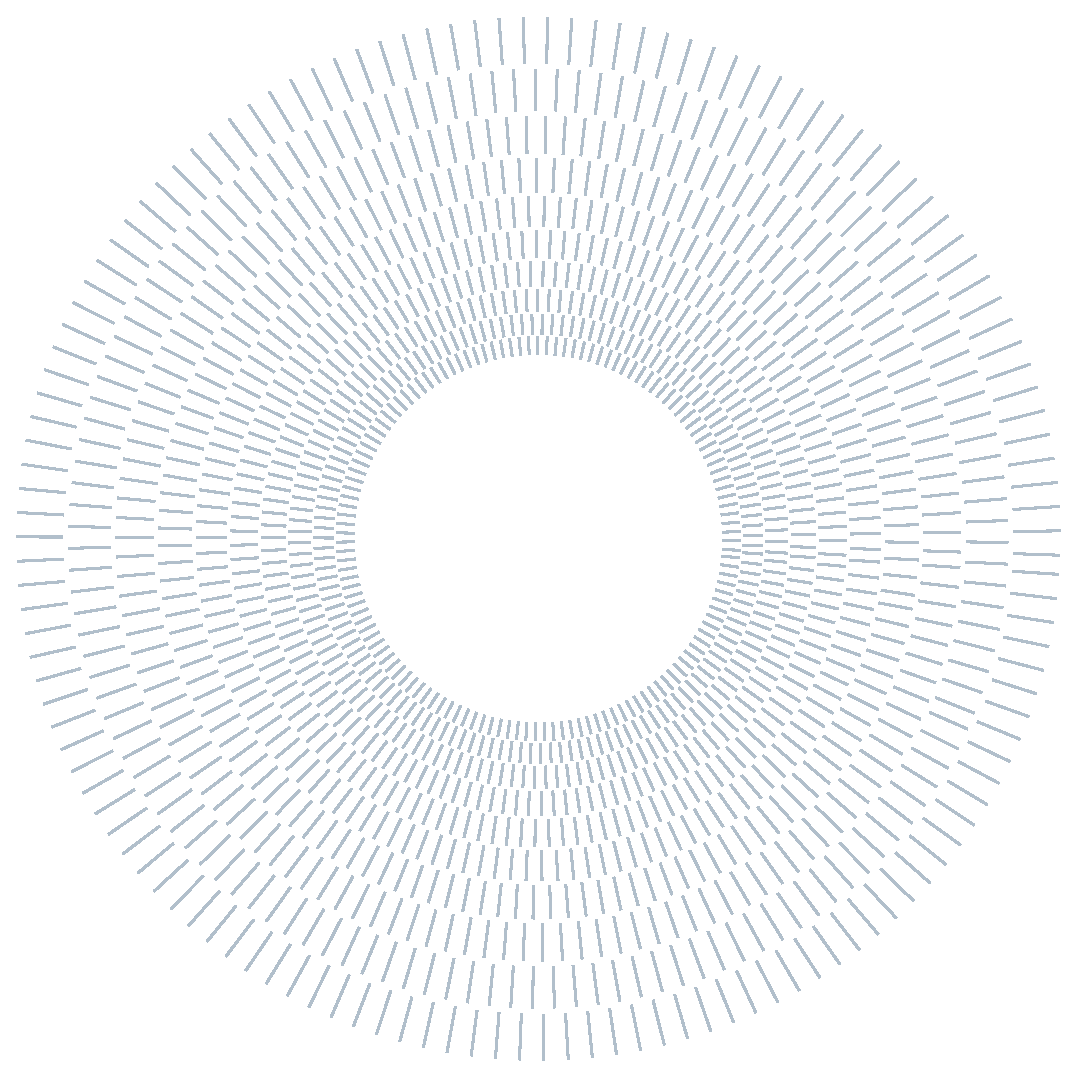
\includegraphics[width=0.44\paperwidth]{raggiera_polimi.eps}%
			\vfill
}}}

% Set indentation
\setlength\parindent{0pt}

% Custom title commands
\titleformat{\section}
{\color{bluePoli}\normalfont\Large\bfseries}
{\color{bluePoli}\thesection.}{1em}{}
\titlespacing*{\section}
{0pt}{2ex}{1ex}

\titleformat{\subsection}
{\color{bluePoli}\normalfont\large\bfseries}
{\color{bluePoli}\thesubsection.}{1em}{}
\titlespacing*{\subsection}
{0pt}{2ex}{1ex}

% Custom headers and footers
\pagestyle{fancy}
\fancyhf{}
      
\fancyfoot{}
\fancyfoot[C]{\thepage} % page
\renewcommand{\headrulewidth}{0mm} % headrule width
\renewcommand{\footrulewidth}{0mm} % footrule width

\makeatletter
\patchcmd{\headrule}{\hrule}{\color{black}\hrule}{}{} % headrule
\patchcmd{\footrule}{\hrule}{\color{black}\hrule}{}{} % footrule
\makeatother

% -> Create the header
\chead[C]{
\centering
\begin{tcolorbox}[arc=0pt, boxrule=0pt, colback=bluePoli!60, width=\textwidth, colupper=white, top=1.7mm, bottom=1.7mm]
    \textbf{Executive summary} \hfill \textbf{\author}  
\end{tcolorbox}
}

%----------------------------------------------------------------------------
%	NEW COMMANDS DEFINED
%----------------------------------------------------------------------------

% EXAMPLES OF NEW COMMANDS
\newcommand{\bea}{\begin{eqnarray}} % Shortcut for equation arrays
\newcommand{\eea}{\end{eqnarray}}
\newcommand{\e}[1]{\times 10^{#1}}  % Powers of 10 notation

%----------------------------------------------------------------------------
%	ADD YOUR PACKAGES (be careful of package interaction)
%----------------------------------------------------------------------------

\usepackage{array,tabularx}
\usepackage{longtable}
\usepackage{multirow}
\usepackage{svg}
\usepackage[utf8]{inputenc}
\usepackage{xcolor}
\usepackage{graphicx,wrapfig} % For figures inside the text
\usepackage{listings} % Show code in text
\usepackage{mdframed} % Example box \begin{example} ... \end{example}

%----------------------------------------------------------------------------
%	ADD YOUR DEFINITIONS AND COMMANDS (be careful of existing commands)
%----------------------------------------------------------------------------

% Better inline code
\definecolor{light-gray}{gray}{0.95}
\newcommand{\inlinecode}[1]{\colorbox{light-gray}{\texttt{#1}}}

% Show code in text
\colorlet{punct}{red!60!black}
\definecolor{CodeBackground}{HTML}{EEEEEE}
\definecolor{delim}{RGB}{20,105,176}
\colorlet{numb}{magenta!60!black}
\lstdefinelanguage{json}{
    basicstyle=\normalfont\ttfamily,
    numbers=left,
    numberstyle=\scriptsize,
    stepnumber=1,
    numbersep=8pt,
    showstringspaces=false,
    breaklines=true,
    frame=lines,
    backgroundcolor=\color{CodeBackground},
    literate=
     *{:}{{{\color{punct}{:}}}}{1}
      {,}{{{\color{punct}{,}}}}{1}
      {\{}{{{\color{delim}{\{}}}}{1}
      {\}}{{{\color{delim}{\}}}}}{1}
      {[}{{{\color{delim}{[}}}}{1}
      {]}{{{\color{delim}{]}}}}{1},
}

% Example box. \begin{example} ... \end{example}
\definecolor{ExampleBoxBackground}{HTML}{999999}
\newmdenv[ % Define mdframe settings and store as leftrule
  linecolor=ExampleBoxBackground,
  linewidth = 2pt,
  topline=false,
  bottomline=false,
  rightline=false,
  skipabove=\topsep,
  skipbelow=\topsep
]{leftrule}
\newenvironment{example}{
	\medskip
	\begin{leftrule}
	\textbf{Example}
	\medskip
	\color{black!60}
   	\newline%
}{
	\medskip
    \end{leftrule}
}

%----------------------------------------------------------------------------
%	BEGIN OF YOUR DOCUMENT
%----------------------------------------------------------------------------

\begin{document}

\fancypagestyle{plain}{%
\fancyhf{} % Clear all header and footer fields
\fancyhead[RO,RE]{\thepage} %RO=right odd, RE=right even
\renewcommand{\headrulewidth}{0pt}
\renewcommand{\footrulewidth}{0pt}}

%----------------------------------------------------------------------------
%	TITLE PAGE
%----------------------------------------------------------------------------

\pagestyle{empty} % No page numbers
\frontmatter % Use roman page numbering style (i, ii, iii, iv...) for the preamble pages

\puttitle{
	title=Location-Aware and Stateful Serverless Computing on the Edge, % Title of the thesis
	name=Dennis Motta, % Author Name and Surname
	course=Computer Science and Engineering, % Study Programme (in Italian)
	ID  = 940064,  % Student ID number (numero di matricola)
	advisor= Alessandro Margara, % Supervisor name
	coadvisor={Gianpaolo Cugola}, % Co-Supervisor name, remove this line if there is none
	academicyear={2020-21},  % Academic Year
} % These info will be put into your Title page 

%----------------------------------------------------------------------------
%	PREAMBLE PAGES: ABSTRACT (inglese e italiano), EXECUTIVE SUMMARY
%----------------------------------------------------------------------------
\startpreamble
\setcounter{page}{1} % Set page counter to 1

% ABSTRACT IN ENGLISH
\chapter{Abstract}

The popularity and proliferation of smart devices (e.g., smartphones, wearable devices, Internet-of-Things sensors) is resulting in an unprecedented growth in the amount of collected data. The current most popular approaches to manage this huge amount of data typically rely on cloud platforms located at the core of the infrastructure.

As the number of devices and the amount of data they generate increases, such core-centric approaches are becoming increasingly inefficient as they need to transfer data back and forth between the core and the devices. Furthermore, the latencies associated with such data transfer are affected by the huge travel-distance needed to make the device communicate to the central cloud platform.

To deal with the aforementioned situation new approaches have been introduced in both academia and industry, exploiting the power of the edge of the network to perform the computation closer to the data source. We noticed a discrepancy between the approaches proposed in research and in industry: research frequently assumes the possibility of running virtual machines or long-running containers on the edge. However, most real-world Web infrastructure companies do not comply with this assumption, due to the limited resource available in the edge.

In this thesis we study the state of the art for stateful computations and data processing on the edge and after carefully analyzing the issues and the needs of the scenario we show the use cases predominantly affected by bandwidth and latency constraints. We then show the current frameworks available in the industry and notice how these solutions do not cover the use cases found. So we then propose a serverless approach effectively applicable by web infrastructure companies, that takes into consideration the problem of the scarcity of the resources while still allowing quite powerful stateful computations on the edge. We also show how we implemented this new approach trough a working prototype, and finally we investigate the gains developers may obtain by using our approach. We demonstrate how several use cases can benefit from this new system though discrete-event simulation, since running our prototype on an emulation of a real global edge network was infeasible due to to sheer amount of resources needed to emulate even a small edge network.

\paragraph{Keywords}  Edge Computing, Serverless, FaaS, Stateful.

% ABSTRACT IN ITALIAN
%\chapter*{Sommario}

La popolarità e la proliferazione di dispositivi intelligenti (e.g., smartphone, dispositivi indossabili, sensori Internet-of-Things) sta determinando una crescita senza precedenti della quantità di dati raccolti. Gli approcci attualmente più diffusi per gestire questa enorme quantità di dati si basano in genere su piattaforme cloud situate al centro dell'infrastruttura.

Con l'aumento del numero di dispositivi e della quantità di dati generati, tali approcci basati su un core centrale stanno diventando sempre più inefficienti poiché devono trasferire i dati avanti e indietro tra il core e i dispositivi. Inoltre, le latenze associate a tale trasferimento di dati sono influenzate dall'enorme distanza di viaggio necessaria per far comunicare il dispositivo con la piattaforma cloud centrale.

Per affrontare la situazione sono stati introdotti nuovi approcci sia nel mondo accademico che nell'industria, sfruttando la potenza dell'edge della rete per eseguire il calcolo più vicino alla fonte dei dati. Abbiamo notato una discrepanza tra gli approcci proposti nella ricerca e nell'industria: la ricerca presuppone spesso la possibilità di eseguire macchine virtuali o container di lunga durata sull'edge. Tuttavia, la maggior parte delle aziende di infrastruttura web non rispettano questa ipotesi a causa delle risorse limitate disponibili nell'edge.

In questa tesi studiamo lo stato dell'arte per le computazioni con stato e per l'elaborazione dei dati sull'edge, e dopo aver analizzato attentamente le problematiche e le esigenze dello scenario mostriamo i casi d'uso prevalentemente affetti da vincoli di larghezza di banda e latenza. Mostriamo quindi i framework attuali disponibili nel settore e notiamo come queste soluzioni non coprono i casi d'uso trovati. Quindi proponiamo un approccio serverless effettivamente applicabile dalle aziende di infrastrutture web, che tenga conto del problema della scarsità delle risorse pur consentendo computazioni stateful abbastanza potenti sull'edge. Mostriamo anche come abbiamo implementato questo nuovo approccio attraverso un prototipo funzionante, e infine esaminiamo i benefici che gli sviluppatori possono ottenere usando il nostro approccio. Dimostriamo come diversi casi d'uso possono trarre vantaggio da questo nuovo sistema attraverso la simulazione a eventi discreti, poiché l'esecuzione del nostro prototipo su un'emulazione di una rete edge globale era impossibile a causa dell'enorme quantità di risorse necessarie per emulare anche una piccola rete edge.

\textbf{Keywords:} Edge Computing, Serverless, FaaS, Stateful


% ACKNOWLEDGEMENTS
\chapter{Acknowledgements}
In this chapter, you can acknowledge the people that were somehow helpful in the realization of the thesis. It is better to keep this chapter formal, you can add the friendly thanks at the end (chapter Thanks).

%----------------------------------------------------------------------------
%	LIST OF CONTENTS/FIGURES/TABLES/SYMBOLS
%----------------------------------------------------------------------------

% TABLE OF CONTENTS
\thispagestyle{empty}
\tableofcontents % Table of contents 
\thispagestyle{empty}
\cleardoublepage

%-------------------------------------------------------------------------
%	THESIS MAIN TEXT
%-------------------------------------------------------------------------
% In the main text of your thesis you can write the chapters in two different ways:
%
%(1) As presented in this template you can write:
%    \chapter{Title of the chapter}
%    *body of the chapter*
%
%(2) You can write your chapter in a separated .tex file and then include it in the main file with the following command:
%    \chapter{Title of the chapter}
%    \input{chapter_file.tex}
%
% Especially for long thesis, we recommend you the second option.

\addtocontents{toc}{\vspace{2em}} % Add a gap in the Contents, for aesthetics
\mainmatter % Begin numeric (1,2,3...) page numbering

% --------------------------------------------------------------------------
% NUMBERED CHAPTERS % Regular chapters following
% --------------------------------------------------------------------------
\chapter{Introduction}

\section{Context}

% This is basically an extension of the abstract. Here you provide context for the problem faced. Keep in mind that even if you now have gained expertise on it, most of the readers are no so inside the problem as you are. Start from the basics and explain clearly. You can also introduce here some hints about the methodology and your contribution. For this purpose, you may also decide to add more sections.

With the increasing number of connected devices and with \gls{IoT} implementation now becoming more widespread, in some cases cloud-centric architectures are starting to be ineffective. Devices are generating a lot of data at the end of the network and many applications are already being deployed at the edge to process the information.
Cisco Systems predicts that an estimated 29 billion devices will connect to the Internet by 2023 \cite{cisco2018-2023}.

Due to the volume, variety and velocity of data generated at the end of the network, the cloud cannot fully support applications that must meet compelling latency or bandwidth constraints: huge distances need to be covered by the communication, increasing the latency and making a large quantity of data pass through the network.
Indeed, the considerable increase in the amount of data produced at the end of the network was not accompanied by a comparable increase of available bandwidth from/to the cloud \cite{promise-of-edge-computing}.

% Furthermore, Cloud connection latencies are not adequate to host real-time tasks such as life-saving connected devices, augmented reality, or gaming [3].

% Some of the applications they run might require very short response times, some might involve private data, and some might produce huge quantities of data. Cloud computing can’t support these IoT applications. Edge computing, on the other hand, can do so and will promote many new IoT applications.

\section{Research Questions}
An increasing trend in edge computing has been found in the last years, however the industry lacks the presence of a stateful development abstraction that allows developers to easily exploit the power of the edge. The absence of this abstraction makes developers still prefer cloud-centric approach despite the related problems.

A non-technology and non-infrastructure dependant framework is needed in order to allow the development of applications with strict constraints of latency and bandwidth.

Therefore this work aims at answering the following research questions (RQ):
\begin{itemize}
    \item[RQ.1]\emph{Which use cases are predominantly affected by bandwidth and latency constraints? What are the common characteristics of these use cases?}
    
    \item[RQ.2]\emph{Which frameworks allowing computation on the edge are currently available in the industry? Can the available frameworks accomplish the use cases seen in RQ.1?}
    
    \item[RQ.3]\emph{Can a new approach accomplish the use cases seen in RQ.1? What are the drawbacks and benefits of the approach?}
\end{itemize}

We use the answers to these questions to propose an innovative framework that allows the developers to abstract away both the infrastructure and the location of the users.

\section{Research Methodology}
TODO

\section{Thesis Outline}
TODO



\iffalse
Here you explain the structure of the thesis.

\begin{example}
The thesis is structured in the following way:
\begin{itemize}
\item In \autoref{ch:preliminaries_and_sota}, we present ... .
\item In \autoref{ch:problem_formulation}, we formulate the problem we address in the thesis and ... .
\item In \autoref{ch:design}, we present our solution for ... .
\item In \autoref{ch:experiments}, we show experimental results of our proposed methods in different settings ... .
\item Finally, in \autoref{ch:conclusions}, we present our conclusions and possible future paths toward which our work could be extended.
\end{itemize}
\end{example}
\fi
\chapter{Preliminaries and State of the Art}
\label{ch:preliminaries_and_sota}
TODO



\iffalse
\section{Preliminary notions}
\label{sec:preliminaries}

\begin{table}[!ht]
\centering
\begin{tabular}{c l} \hline
\textbf{Notation}&\textbf{Description} \\ \hline
$G$&Graph\\
$V$&set of nodes of $G$\\
$E$&set of edges of $G$\\
$W$&set of weights corresponding to each edge in $E$\\
$w_{u,v}$&weight of edge $(u,v)$\\
$n$&$|V|$, number of nodes\\
$m$&$|E|$, number of edges\\
\hline
\end{tabular}
\caption{Graph notation.}
\label{tab:notation}
\end{table}

``In this section, we introduce the preliminary notions at the base of our study. We start by briefly introducing the problem, and then we provide the necessary concepts and the notation used."

You may insert a subsection for each of the most relevant features of your problem. You can add some reference if needed, but just to explain the problem. The references with the solutions of the problem should be put in the next section.

You can keep a notation table for the notation used in this chapter as \autoref{tab:notation}. Everything inside the notation table must be written at least once inside this chapter. You can put an extended notation for the whole thesis in the appendix.

It is likely that you have to present definitions, theorems or propositions. We suggests to use the environments provided by the template. You can find the guide in the LaTeX suggestions chapter.

\section{State of the Art}
\label{sec:sota}

In this section, we survey the most relevant works related to the argument of your thesis. If you face a problem that has more than one macro-topic, you may choose to add a subsection for each of these topics (better no more than 2-3), like \emph{Related works on Topic 1}, etc.

List the works in chronological order and cite only the most important and pertinent ones, avoid 100 citations for a master thesis.
\fi

%\chapter{Chapter one}
\label{ch:chapter_one}%
% The \label{...}% enables to remove the small indentation that is generated, always leave the % symbol.

In this chapter additional useful information are reported.

\section{Sections and subsections}
\label{sec:section_name}
Chapters are typically subdivided into sections and subsections, and, optionally,
subsubsections, paragraphs and subparagraphs.
All can have a title, but only sections and subsections are numbered.
A new section is created by the command
\begin{verbatim}
\section{Title of the section}
\end{verbatim}
The numbering can be turned off by using \verb|\section*{}|.
\\
A new subsection is created by the command
\begin{verbatim}
\subsection{Title of the subsection}
\end{verbatim}
and, similarly, the numbering can be turned off by adding an asterisk as follows 
\begin{verbatim}
\subsection*{}
\end{verbatim}

\section{Equations}
\label{sec:eqs}
This section gives some examples of writing mathematical equations in your thesis.

Maxwell's equations read:
\begin{subequations}
    \label{eq:maxwell}
    \begin{align}[left=\empheqlbrace]
    \nabla\cdot \bm{D} & = \rho, \label{eq:maxwell1} \\
    \nabla \times \bm{E} +  \frac{\partial \bm{B}}{\partial t} & = \bm{0}, \label{eq:maxwell2} \\
    \nabla\cdot \bm{B} & = 0, \label{eq:maxwell3} \\
    \nabla \times \bm{H} - \frac{\partial \bm{D}}{\partial t} &= \bm{J}. \label{eq:maxwell4}
    \end{align}
\end{subequations}

Equation~\eqref{eq:maxwell} is automatically labeled by \texttt{cleveref},
as well as Equation~\eqref{eq:maxwell1} and Equation~\eqref{eq:maxwell3}.
Thanks to the \verb|cleveref| package, there is no need to use \verb|\eqref|.
Remember that Equations have to be numbered only if they are referenced in the text.

Equations~\eqref{eq:maxwell_multilabels1}, \eqref{eq:maxwell_multilabels2}, \eqref{eq:maxwell_multilabels3}, and \eqref{eq:maxwell_multilabels4} show again Maxwell's equations without brace:
\begin{align}
    \nabla\cdot \bm{D} & = \rho, \label{eq:maxwell_multilabels1} \\
    \nabla \times \bm{E} +  \frac{\partial \bm{B}}{\partial t} &= \bm{0}, \label{eq:maxwell_multilabels2} \\
    \nabla\cdot \bm{B} & = 0, \label{eq:maxwell_multilabels3} \\
    \nabla \times \bm{H} - \frac{\partial \bm{D}}{\partial t} &= \bm{J} \label{eq:maxwell_multilabels4}.
\end{align}

Equation~\eqref{eq:maxwell_singlelabel} is the same as before,
but with just one label:
\begin{equation}
    \label{eq:maxwell_singlelabel}
    \left\{
    \begin{aligned}
    \nabla\cdot \bm{D} & = \rho, \\
    \nabla \times \bm{E} +  \frac{\partial \bm{B}}{\partial t} &= \bm{0},\\
    \nabla\cdot \bm{B} & = 0, \\
    \nabla \times \bm{H} - \frac{\partial \bm{D}}{\partial t} &= \bm{J}.
    \end{aligned}
    \right.
\end{equation}

\section{Figures, Tables and Algorithms}
Figures, Tables and Algorithms have to contain a Caption that describe their content, and have to be properly reffered in the text.

\subsection{Figures}
\label{subsec:figures}

For including pictures in your text you can use \texttt{TikZ} for high-quality hand-made figures,
or just include them as usual with the command
\begin{verbatim}
\includegraphics[options]{filename.xxx}
\end{verbatim}
Here xxx is the correct format, e.g. \verb|.png|, \verb|.jpg|, \verb|.eps|, \dots.

\begin{figure}[H]
    \centering
    
\includegraphics[width=0.3\textwidth]{logo_polimi_scritta.eps}
    \caption{Caption of the Figure to appear in the List of Figures.}
    \label{fig:quadtree}
\end{figure}

Thanks to the \texttt{\textbackslash subfloat} command, a single figure, such as Figure~\ref{fig:quadtree},
can contain multiple sub-figures with their own caption and label, e.g. \color{black} Figure~\ref{fig:polimi_logo1} and Figure~\ref{fig:polimi_logo2}. 

\begin{figure}[H]
    \centering
    \subfloat[One PoliMi logo.\label{fig:polimi_logo1}]{
        
\includegraphics[scale=0.5]{Images/logo_polimi_scritta.eps}
    }
    \quad
    \subfloat[Another one PoliMi logo.\label{fig:polimi_logo2}]{
        
\includegraphics[scale=0.5]{Images/logo_polimi_scritta2.eps}
    }
    \caption[Shorter caption]{This is a very long caption you don't want to appear in the List of Figures.}
    \label{fig:quadtree2}
\end{figure}


\subsection{Tables}
\label{subsec:tables}

Within the environments \texttt{table} and  \texttt{tabular} you can create very fancy tables as the one shown in Table~\ref{table:example}.
\begin{table}[H]
    \caption*{\textbf{Title of Table (optional)}}
    \centering 
    \begin{tabular}{|p{3em} c c c |}
    \hline
    \rowcolor{bluepoli!40} % comment this line to remove the color
     & \textbf{column 1} & \textbf{column 2} & \textbf{column 3} \T\B \\
    \hline \hline
    \textbf{row 1} & 1 & 2 & 3 \T\B \\
    \textbf{row 2} & $\alpha$ & $\beta$ & $\gamma$ \T\B\\
    \textbf{row 3} & alpha & beta & gamma \B\\
    \hline
    \end{tabular}
    \\[10pt]
    \caption{Caption of the Table to appear in the List of Tables.}
    \label{table:example}
\end{table}

You can also consider to highlight selected columns or rows in order to make tables more readable.
Moreover, with the use of \texttt{table*} and the option \texttt{bp} it is possible to align them at the bottom of the page. One example is presented in Table~\ref{table:exampleC}. 

\begin{table}[H]
\centering 
    \begin{tabular}{|p{3em} | c | c | c | c | c | c|}
    \hline
%    \rowcolor{bluepoli!40}
     & \textbf{column1} & \textbf{column2} & \textbf{column3} & \textbf{column4} & \textbf{column5} & \textbf{column6} \T\B \\
    \hline \hline
    \textbf{row1} & 1 & 2 & 3 & 4 & 5 & 6 \T\B\\
    \textbf{row2} & a & b & c & d & e & f \T\B\\
    \textbf{row3} & $\alpha$ & $\beta$ & $\gamma$ & $\delta$ & $\phi$ & $\omega$ \T\B\\
    \textbf{row4} & alpha & beta & gamma & delta & phi & omega \B\\
    \hline
    \end{tabular}
    \\[10pt]
    \caption{Highlighting the columns}
    \label{table:exampleC}
\end{table}

\begin{table}[H]
\centering 
    \begin{tabular}{|p{3em} c c c c c c|}
    \hline
%    \rowcolor{bluepoli!40}
     & \textbf{column1} & \textbf{column2} & \textbf{column3} & \textbf{column4} & \textbf{column5} & \textbf{column6} \T\B \\
    \hline \hline
    \textbf{row1} & 1 & 2 & 3 & 4 & 5 & 6 \T\B\\
    \hline
    \textbf{row2} & a & b & c & d & e & f \T\B\\
    \hline
    \textbf{row3} & $\alpha$ & $\beta$ & $\gamma$ & $\delta$ & $\phi$ & $\omega$ \T\B\\
    \hline
    \textbf{row4} & alpha & beta & gamma & delta & phi & omega \B\\
    \hline
    \end{tabular}
    \\[10pt]
    \caption{Highlighting the rows}
    \label{table:exampleR}
\end{table}

\subsection{Algorithms}
\label{subsec:algorithms}

Pseudo-algorithms can be written in \LaTeX{} with the \texttt{algorithm} and \texttt{algorithmic} packages.
An example is shown in Algorithm~\ref{alg:var}.
\begin{algorithm}[H]
    \label{alg:example}
    \caption{Name of the Algorithm}
    \label{alg:var}
    \label{protocol1}
    \begin{algorithmic}[1]
    \STATE Initial instructions
    \FOR{$for-condition$}
    \STATE{Some instructions}
    \IF{$if-condition$}
    \STATE{Some other instructions}
    \ENDIF
    \ENDFOR
    \WHILE{$while-condition$}
    \STATE{Some further instructions}
    \ENDWHILE
    \STATE Final instructions
    \end{algorithmic}
\end{algorithm} 

\vspace{5mm}

\section{Theorems, propositions and lists}

\subsection{Theorems}
Theorems have to be formatted as:
\begin{theorem}
\label{a_theorem}
Write here your theorem. 
\end{theorem}
\textit{Proof.} If useful you can report here the proof.

\subsection{Propositions}
Propositions have to be formatted as:
\begin{proposition}
Write here your proposition.
\end{proposition}

\subsection{Lists}
How to  insert itemized lists:
\begin{itemize}
    \item first item;
    \item second item.
\end{itemize}
How to insert numbered lists:
\begin{enumerate}
    \item first item;
    \item second item.
\end{enumerate}

\section{Use of copyrighted material}

Each student is responsible for obtaining copyright permissions, if necessary, to include published material in the thesis.
This applies typically to third-party material published by someone else.

\section{Plagiarism}

You have to be sure to respect the rules on Copyright and avoid an involuntary plagiarism.
It is allowed to take other persons' ideas only if the author and his original work are clearly mentioned.
As stated in the Code of Ethics and Conduct, Politecnico di Milano \textit{promotes the integrity of research,
condemns manipulation and the infringement of intellectual property}, and gives opportunity to all those
who carry out research activities to have an adequate training on ethical conduct and integrity while doing research.
To be sure to respect the copyright rules, read the guides on Copyright legislation and citation styles available
at:
\begin{verbatim}
https://www.biblio.polimi.it/en/tools/courses-and-tutorials
\end{verbatim}
You can also attend the courses which are periodically organized on "Bibliographic citations and bibliography management".

\section{Bibliography and citations}
Your thesis must contain a suitable Bibliography which lists all the sources consulted on developing the work.
The list of references is placed at the end of the manuscript after the chapter containing the conclusions.
We suggest to use the BibTeX package and save the bibliographic references  in the file \verb|Thesis_bibliography.bib|.
This is indeed a database containing all the information about the references. To cite in your manuscript, use the \verb|\cite{}| command as follows:
\\
\textit{Here is how you cite bibliography entries: \cite{knuth74}, or multiple ones at once: \cite{knuth92,lamport94}}.
\\
The bibliography and list of references are generated automatically by running BibTeX \cite{bibtex}.
\chapter{Problem formulation}
\label{ch:problem_formulation}

This chapter is dedicated to the formal presentation of the problem with the technical details. Here your should put also the figure of merit you use to compare your solution with the ones of the related works you presented.

\begin{example}
In this thesis, we address the problem of ... . [Description of the problem and classical approaches]. The figure of merit we use to compare the solutions is ... .
\end{example}

\chapter{Design of the Solution}
\label{ch:design}

Let’s imagine a global infrastructure with many edge locations. Some web infrastructure companies already provide a network with many locations, like the one of Cloudflare with more than 250 locations worldwide located in more than 100 different countries \cite{cloudflare-network}, or the network of Amazon Web Services (AWS) with more than 265 edge locations \cite{aws-network}.
These networks are only the beginning of the development of edge networks: AWS is currently introducing AWS Wavelength \cite{aws-wavelength} a new service in partnership with popular telecommunication providers (i.e., Verizon, Vodafone) to scale across global 5G networks.


\section{Managing the network}
By having such a vast and heterogeneous network the first step in our approach is to abstract away the difficult management of the deployment to the many edge locations.
In a traditional cloud setup the developer specifies individually on which data center to deploy, this cannot be done efficiently for a vast edge network because the developer would have to specify hundreds of specific deployments.
The developer could also want to use only more powerful data centers and not the limited cloudlets at the border of the network.

\begin{wrapfigure}[11]{r}{5.5cm} % [11] is how many lines should be wrapped
\caption{An example of the hierarchy.}
\label{fig:hierarchy}
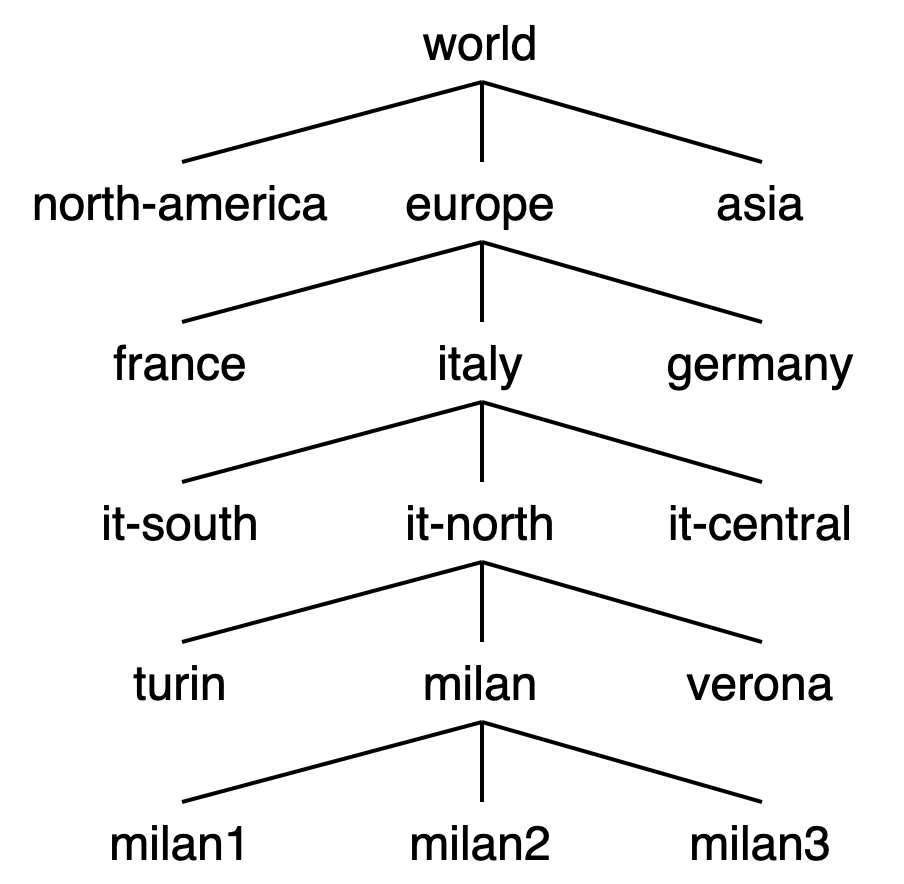
\includegraphics[width=5.5cm]{Figures/Solution/hierarchy.png}
\end{wrapfigure} 

To allow flexibility in the deployments and, as we will see later, to allow geographical aggregations we can organize the various machines running in the data centers and cloudlets in a hierarchy with multiple levels.
In Figure \ref{fig:hierarchy} we reported an example: we first have a division by continent (or large regions), then by country, territory, city and district.
Note that each element in the hierarchy should not necessarily be a different data center: a big data center in Milan can be both a receiver for "city" and "country" deployments/aggregations.
\vspace{0.5cm}


\subsection{Specifying locations}
The job of specifying the available locations should be responsibility of the web infrastructure company, but still the developer may want to customize the arrangement or may want to use their personal infrastructure. 

So we must provide a way to specify the hierarchy, we chose to implement the API in the following way:
\begin{itemize}
    \item Levels: the list of levels characterized by their identifiers (e.g., "continent", "country", "territory", "city", "district");
    \item Hierarchy: a way to specify the hierarchy, starting from the uppermost level and going down to the lowest level. Each level can contain multiple locations, and each location will aggregate data of the relative area;
    \item Location: each location must be associated to an entry point that defines the actual cloudlet or data center to be used (so for the location there must be defined gateway, port and password).
\end{itemize}

TODO show constraints


\subsection{Specifying deployments}
Now that we have the hierarchy specified we can use this hierarchy to make a powerful deployment API. The developer should be able to deploy on a specific level of the hierarchy only in a certain area and to exclude a specific subsection from this area.

To allow such deployment we established the following concepts:
\begin{itemize}
    \item \inlinecode{inEvery}: a string representing the level on which to deploy the function.
    \item \inlinecode{inAreas}: a list of string of areas, specifying in which areas to deploy. If unspecified we can assume the developer wants it deployed everywhere. 
     \item \inlinecode{exceptIn}: a list of string of areas, that are an exception to what previously defined before. In the locations contained in these areas the developer does not want to perform the deployment.
\end{itemize}

\begin{example}
Deploy on every city in Europe and Asia, excluding the cities in Italy and excluding the city of Tokyo.
Becomes:
\begin{itemize}
    \item \inlinecode{inEvery}: "city"
    \item \inlinecode{inAreas}: ["europe", "asia"]
     \item \inlinecode{exceptIn}: ["italy", "tokyo"]
\end{itemize}
\end{example}

\begin{example}
Deploy on every district in Europe and India, excluding the districts in France and excluding the districts in Milan.
Becomes:
\begin{itemize}
    \item \inlinecode{inEvery}: "district"
    \item \inlinecode{inAreas}: ["europe", "india"]
     \item \inlinecode{exceptIn}: ["france", "milan"]
\end{itemize}
\end{example}

In the examples we saw that the developer should also be allowed to mix the levels of the areas specified, using different levels of the hierarchy inside the \inlinecode{inAreas} and \inlinecode{exceptIn} lists.

TODO show constraints


\section{Managing limited resources}
Usually edge locations have limited resources compared to central data centers, so web infrastructure companies have to work around the limitations in order to provide a reliable service.
Due to these limitations, Function-as-a-Service (FaaS) is the current de facto standard for companies that provide computing resources at the edge to the public. Examples of services are AWS Lambda@Edge (an evolution of the famous AWS Lambda service on the cloud) \cite{aws-lambda-at-edge} or Cloudflare Workers \cite{cloudflare-workers}. It can be easily understood that providing Infrastructure-as-a-Service (IaaS) or Platform-as-a-Service (PaaS) to the public on the limited resources available at the edge is clearly less efficient for companies.

Therefore we decided to use in our framework the FaaS paradigm as a way to allow the users of the framework (the developers) to perform computation on the edge. The developer, should also be able to specify the RAM memory allocated for the function. The default allocated memory can be a low value, but if there is a more complex function requiring additional memory usage the developer can change the allocated memory (the web infrastructure company can then charge more based on the memory requested).

But resources are not only limited in the sense of computation, but also the storage resources are limited on the edge. To take into account the aforementioned issue we decided to use a key-value database for the stateful part of our approach. A key-value database allows us to perform extremely efficient (but simple) queries, and is perfect for the limited resources available on the edge. To avoid to accumulate data we also introduced in our framework a Time-To-Live (TTL) which the developer must specify. For example with a TTL of 5 days, after making a write to the database the data, if not updated, can be deleted after 5 days.


\subsection{Writing data}
Our goal is to provide the developers an easy way to create geographical aggregations of data. If for the data it does not make sense to create geographical aggregations then it would make more sense to use a core-centric approach to manage this data. In our approach by having the data geographically distributed it means that those data correspond to information coming from the respective geographic area.

Furthermore in Chapter \ref{ch:problem_formulation} we outlined use cases which are static in the sense of location, or for which having discontinuity in the data is not a problem. Therefore we decided to not introduce any session consistency to avoid the cost of managing such sessions: heavy communications between the locations. This means that if we are performing a "city" aggregation and a client that is sending data is currently travelling and changes its position to a new "city" area, then its old data will remain the in the previous "city" area and not transferred to the new one.

To manage such conditions our approach should have the following properties:
\begin{itemize}
    \item Write Action: the action to perform for writing data (e.g., set, add to list, ...)
    \item Key: The key that will be associated to the value as in a standard key-value database.
     \item Data: the data to be associated to the key (so it can be then obtained from the key) or the data to be added to the list specified by the key.
     \item Referring Area Level: the higher level on which to aggregate the data.
     \item Should Save In Intermediate Levels: a true or false property that if set to true saves the data only in the level specified by the Referring Area Level, otherwise the data is saved on the receiving level and on all the other upper levels, up until the level specified by Referring Area Level.
     \item Time To Live: limits the lifespan of the data.
\end{itemize}

To provide some examples, in the code that will be deployed on the "city" level the developer can make the following write calls:

\begin{example}
\begin{itemize}
    \item Write Action: set
    \item Key: mykey1
    \item Data: data1
    \item Referring Area Level: continent
    \item Should Save In Intermediate Levels: false
    \item Time To Live: 10 days
\end{itemize}
The framework will save the data only at the continent level (so if the code is executed in the "milan" location, the data will be saved in the "europe" location). The framework will create (or update) key "mykey1" with the value "data1" and will set a lifespan of the data to 10 days.
\end{example}

\begin{example}
\begin{itemize}
    \item Write Action: set
    \item Key: mykey2
    \item Data: data2
    \item Referring Area Level: continent
    \item Should Save In Intermediate Levels: true
    \item Time To Live: 30 days
\end{itemize}
The framework will save the data at the continent, country, territory and city levels (so if the code is executed in the "milan" location, the data will be saved in the "it-north", "italy" and "europe" locations). In each of these locations the framework will create (or update) key "mykey2" with the value "data2" and will set a lifespan of the data to 30 days.
\end{example}

\begin{example}
\begin{itemize}
    \item Write Action: add to list
    \item Key: mylist1
    \item Data: data1
    \item Referring Area Level: continent
    \item Should Save In Intermediate Levels: false
    \item Time To Live: 1 day
\end{itemize}
The framework will save the data only at the continent level (so if the code is executed in the "milan" location, the data will be saved in the "europe" location). The framework will add to the list associated to the key "mylist1" the value "data1" and will set a lifespan to the single element of the list 1 day.
\end{example}


\subsection{Reading data}
As we have seen the developer has to think carefully how to handle the writing of the data with the objective to partition geographically the data. But after data have been thoughtfully partitioned then the reading of the data is instantaneous.
When running the code in a certain location, by specifying only the reading action and key the framework obtains the data present in the location and associated to that key.

So only the following two properties are use for making reads:
\begin{itemize}
    \item Read Action: the action to perform for reading data, "get" to obtain the single value from the key (saved with "set"), "get list" to obtain all the values saved with "add to list".
    \item Key: The key of the value or the list to be read.
\end{itemize}

To provide some examples, in the code that will be deployed on the "continent" level, for reading the data saved in that "continent" location (e.g., "europe" location) the developer can make the following read calls:
\begin{example}
\begin{itemize}
    \item Read Action: get
    \item Key: mykey1
\end{itemize}
The framework will obtain the value associated to the key "mykey1" if present and if not expired due to the TTL.
\end{example}

\begin{example}
\begin{itemize}
    \item Read Action: get list
    \item Key: mylist1
\end{itemize}
The framework will obtain all the not expired elements contained in the list associated to the key "mylist1".
\end{example}


\section{Applying to use cases}
TODO show how these APIs can be used in a few use cases











\iffalse
``This approach is similar to the one proposed in a recent work by Nuara et al.~\cite{nuara2020driving}, in which ..."
\fi

\chapter{The Prototype}
\label{ch:prototype}

In this chapter we will show the implementation of the prototype running the API that we presented in the previous chapter.

\section{The FaaS platform}
We saw in Chapter \ref{ch:preliminaries_and_sota} the State of the Art for FaaS platforms, we saw a very valid implementation focused on edge use cases like the one of Cloudflare Workers but unfortunately, being a proprietary solution, it cannot be applied in our framework.
So we resorted to an open source solution and we chose the solution provided by OpenFaaS since they provide two versions of their system, one version for high-performing machines with more overhead but that can scale greatly, and another more efficient version for edge devices with a smaller overhead but that cannot scale horizontally (there can only be one replica of the container running the function).

We implemented two FaaS triggers in our prototype: an HTTP trigger (a trigger that gets activated by a simple HTTP request) and the cron trigger (a trigger that is automatically called periodically based on the current time).


\subsection{Specifying locations}
We provided a way to specify the hierarchy associated to the infrastructure by using the JavaScript Object Notation format (JSON).
Below we provide an example of a hierarchy with 4 levels: continent, country, city, district.

\begin{lstlisting}[language=json,firstnumber=1]
{
  "areaTypesIdentifiers": ["continent", "country", "city", "district"],
  "hierarchy": {
    "europe": {
      "main-location": { },
      "italy": {
        "main-location": { },
        "milan": {
          "main-location": { },
          "milan001": { },
          "milan002": { }
        },
        "turin": {
          "main-location": { },
          "turin001": { },
          "turin002": { }
        }
      },
      "france": {
        "main-location": { },
        "paris": {
          "main-location": { },
          "paris001": { },
          "paris002": { }
        },
        "nice": {
          "main-location": { },
          "nice001": { },
          "nice002": { }
        }
      }
    }
  }
}
\end{lstlisting}

So we used the hierarchical structure of JSON to represent the infrastructure hierarchy. In this example we have one "continent" location called "europe", containing two "country" locations called "italy" and "france", containing four "city" locations called "milan", "turin", "paris" and "nice", in turn containing eight "district" locations.

The details of the locations and the way to communicate with them are not reported in this example, but these information must be written in the places where two empty braces \inlinecode{\{ \}} are present.
\chapter{Experimental evaluation}
\label{ch:experiments}

In this chapter, we present experimental results on the system proposed. Two types of evaluations are present: a first assessment done on the working prototype running on multiple \glspl{VM} and an evaluation of the performance of the approach, measured using a simulation run on a discrete-event simulator.
In the first case, since it's not possible to emulate a network similar to a real edge network due to the amount of resources needed, we focus on the effectiveness, efficiency and usability of the framework.
While with the discrete-event simulation at hand we can focus on the performance obtained and the resources consumed.
In both scenarios we compare the proposed approach to a typical core-centric approach.



\section{Emulation}
TODO



\section{Simulation}
Using a popular discrete-event simulator written in Python, called SimPy \cite{simpy}, we developed a simulation of our approach. Then we compared our approach with the simulation of a core-centric approach.


\subsection{Components}
To simulate the framework we developed the following abstract components in SimPy:
\begin{itemize}
    \item \inlinecode{Client}: a simplified abstraction of a machine that simply sends or requests data;
    \item \inlinecode{Transmission}: a simplified abstraction of a virtual link between two machines;
    \item \inlinecode{ProcessingUnit}: a simplified abstraction of a machine that performs a processing job;
\end{itemize}

In the following section we see in the details the behaviour of these abstract components, and their respective realization.


\subsubsection{Client}
There are two realizations of the \inlinecode{Client} abstract component:
\begin{itemize}
    \item \inlinecode{DataProducerClient}: produces a message with a significant amount of data and always sends the message in a deterministic way to a single \inlinecode{ProcessingUnit} (when simulating our edge approach it sends the message to the lowest level of the hierarchy);
    \item \inlinecode{DataReaderClient}: that produces a message with a small amount of data, this message is used to simulate the retrieval of aggregated data. In the edge scenario the level contacted to make the read request can be any level of the hierarchy.
\end{itemize}


\subsubsection{Transmission}
The \inlinecode{Transmission} component allows to simulate the communication between a \inlinecode{Client} and a \inlinecode{ProcessingUnit} or between two \inlinecode{ProcessingUnit} components.
The \inlinecode{Transmission} is initialized with two inputs: the information about the distance between the two machines and a boolean value (\inlinecode{is\_weak\_network}) specifying if the communication passes through only the faster backbone network. The job of the \inlinecode{Transmission} component is converting the two inputs into a single value of latency and simulating this latency.

To compute the latency the \inlinecode{Transmission} component does as follows:

\[ latency = network\_delay +  distance\_delay \]

\[
    network\_delay= 
\begin{cases}
    weak\_network\_delay,    & \text{if } is\_weak\_network\\
    robust\_network\_delay,  & \text{otherwise}
\end{cases}
\]

\[ distance\_delay = \frac{distance}{SPEED\_OF\_SIGNAL} \]

The \inlinecode{network\_delay} is a value representing a constant latency toll that needs to be paid when making the communication, this value simply depends on the \inlinecode{is\_weak\_network} boolean. The network which is used by the client (i.e., Wi-Fi, LTE, copper cables) is considered to be weak.

The \inlinecode{distance\_delay} is a value that is proportional to the distance that the signal needs to travel.

The constant \inlinecode{SPEED\_OF\_SIGNAL} is computed in the following way:

\[ SPEED\_OF\_SIGNAL = c \cdot 0.67 \cdot 0.50 \cdot \frac{1}{\sqrt{2}} \]

Where \inlinecode{c} is the speed of light in a vacuum; 0.67 denotes how fast a signal travels through the optical fiber media \cite{optical-fiber-latency}; 0.50 is used to take into consideration the round trip time; \(\frac{1}{\sqrt{2}}\) ($\approx$0.707) is used to take into consideration the fact that cables cannot make a direct path between two points, this offset allows us to put as input the straight line distance between two points.


\subsubsection{ProcessingUnit}
A \inlinecode{ProcessingUnit} component waits for data coming from a \inlinecode{Transmission} component. When new data arrives it is put in an unbounded queue that is used by the cores for starting the processes, so by having \textit{N} cores it means that the \inlinecode{ProcessingUnit} can execute \textit{N} processes in parallel.
When a core is free it takes as input the data from the queue and starts simulating the data processing. The simulation time needed for the data processing is computed as the sum of \inlinecode{start\_delay} and \inlinecode{time\_to\_process}. The value of \inlinecode{start\_delay} is used to simulate a constant delay needed to start the processing and initializing the required resources, while \inlinecode{time\_to\_process} is a value that is computed as:

\[ time\_to\_process = \frac{megabytes\_of\_data}{bandwidth\_capability} \]

Where \inlinecode{megabytes\_of\_data} represents the quantity of data sent in the message and \inlinecode{bandwidth\_capability} represents the Megabytes per unit of time that the core can process. As we will see, a core of an edge device is assumed to be less performing than a core in a big cloud data-center.

The realizations of \inlinecode{ProcessingUnit} are shown below in Figure \ref{fig:processing-unit-realizations}.

\begin{figure}[H]
    \centering
    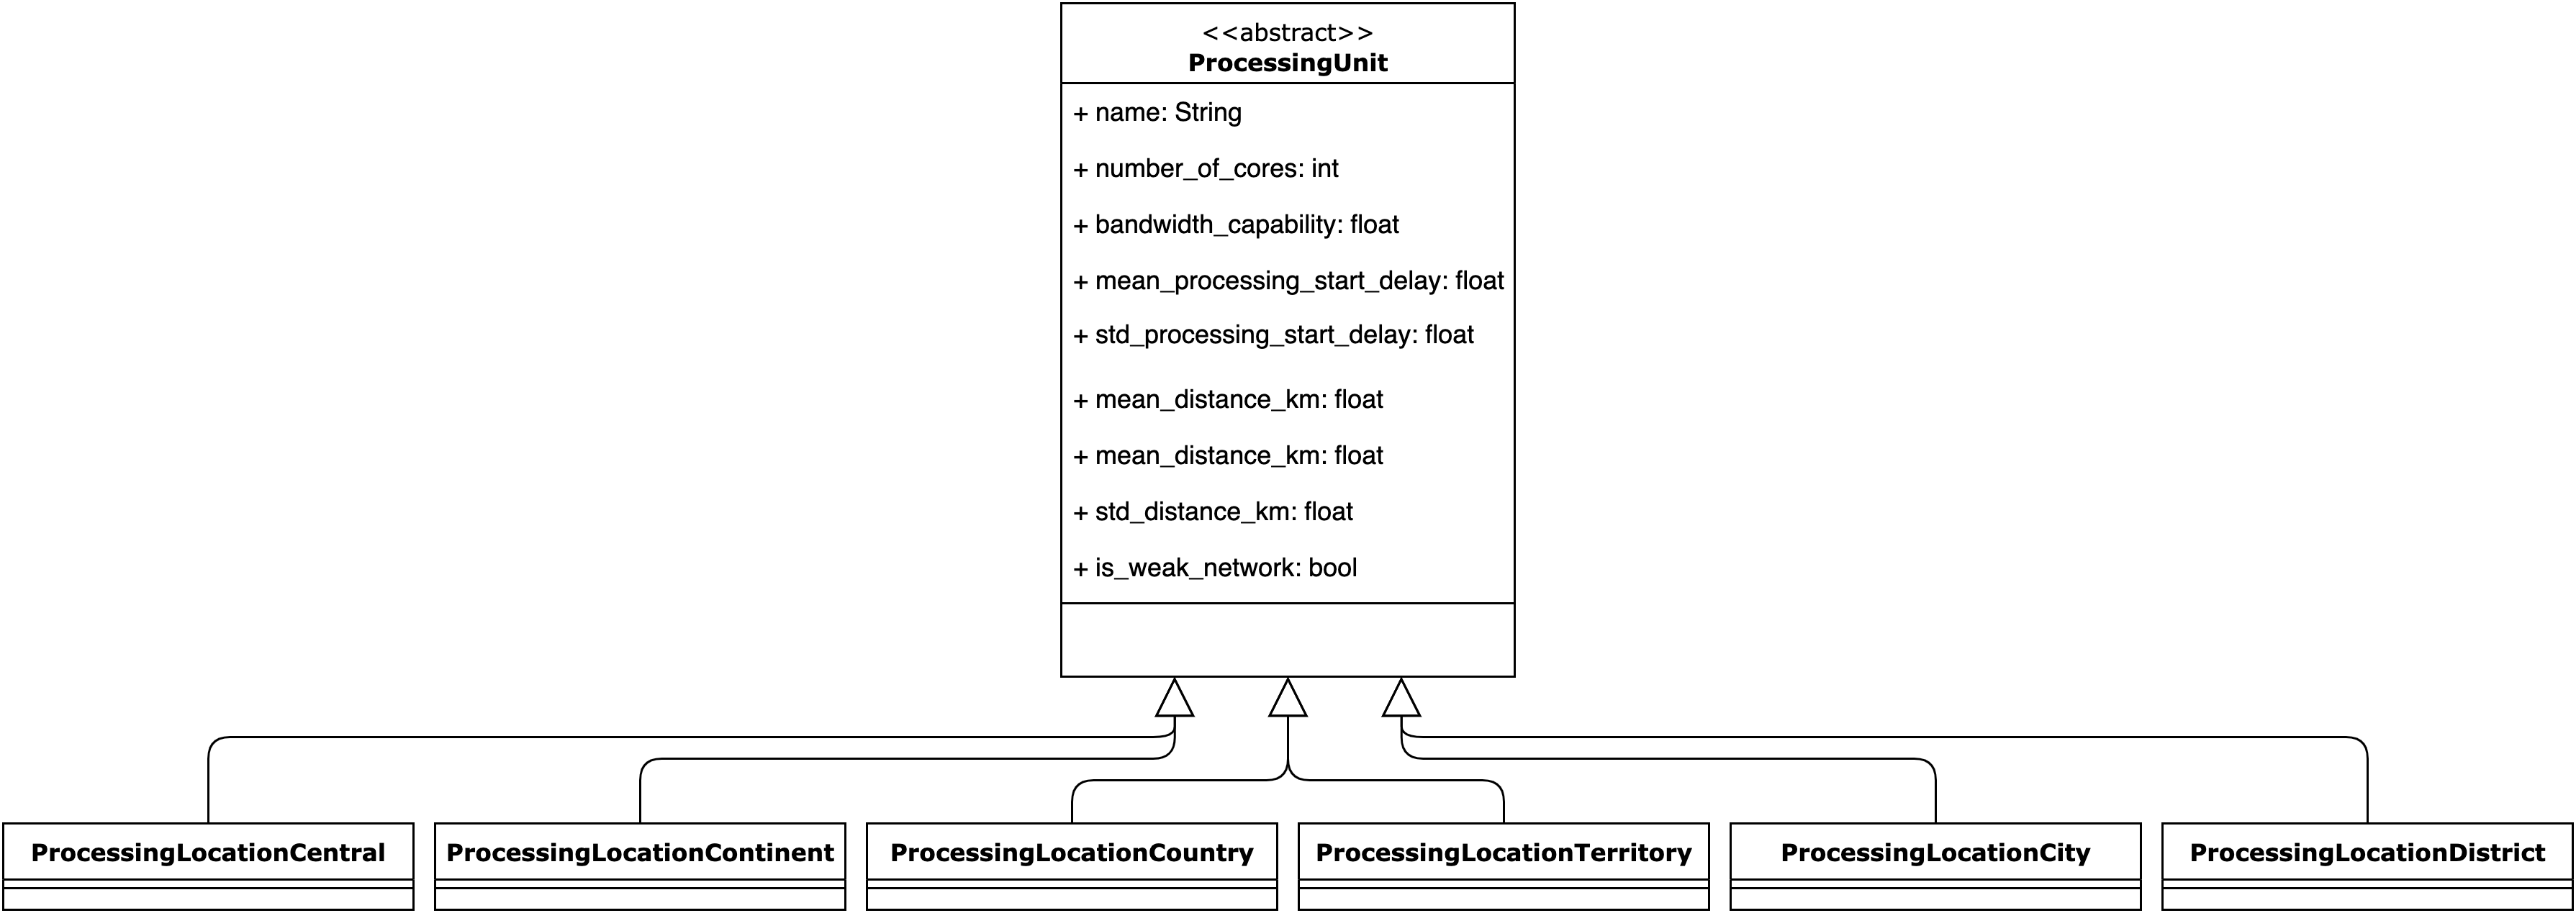
\includegraphics[width=0.66\linewidth]{Figures/Evaluation/processing-unit-realizations.png}
    \caption{Concrete realizations of the ProcessingUnit component.}
    \label{fig:processing-unit-realizations}
\end{figure}


\subsection{Matching the abstractions to a real use case}
To better narrow down the abstractions we can see in one of our use cases how these abstractions match a real scenario: in the traffic use case (TODO ref to use case chapter) the \inlinecode{DataProducerClient} represents the camera producing frames of the road. In our edge scenario the camera sends the frame to the lowest level in the hierarchy, which in our example architecture correspond to the "district" level (\inlinecode{ProcessingLocationDistrict}). While in the core-centric scenario the camera sends the frame to the central cloud (\inlinecode{ProcessingLocationCentral}).

The action of sending the frame is simulated using the \inlinecode{Transmission} component. The frame is then processed by applying an image recognition algorithm, an algorithm which is simulated as a data processing by the receiving \inlinecode{ProcessingUnit}.

In the core-centric scenario the output data is ready when finished processing. While in our edge scenario the ouput data is sent to the specified aggregating \inlinecode{ProcessingUnit} which needs to save the data. The communication is again simulated using the \inlinecode{Transmission} component, while the saving of data is simulated as a small processing of data in the aggregating \inlinecode{ProcessingUnit}.

A client can then need to know the traffic in a specific area. This is simulated using the \inlinecode{DataReaderClient} component which can send a read request message, sent using the \inlinecode{Transmission} component and processed by the receiving \inlinecode{ProcessingUnit}.


\subsection{Simulation Setting}
\label{section:simulation_setting}
Since the setting is similar in the various experiments, we present in the tables below the default values of the variables used in the experiments. The actual value will be extracted case by case from a normal distribution truncated to the left at zero. If the standard deviation is zero the value is actually a constant. Unless specified otherwise the values specified here are the ones used in the experiments.

\begin{table}[H]
\centering
\begin{tabular}{|c|c|l|}
\hline
\textbf{Variable}                                               & \textbf{Mean}              & \textbf{Standard deviation} \\ \hline
\begin{tabular}[c]{@{}c@{}}Number of clients\end{tabular}       & 2000                       & 0                           \\ \hline
\begin{tabular}[c]{@{}c@{}}Time between requests\end{tabular}   & 10s                        & 3s                          \\ \hline
\begin{tabular}[c]{@{}c@{}}Message size\end{tabular}            & 423KB                      & 150KB                       \\ \hline
\end{tabular}
\caption{Default values for variables of DataProducerClient}
\label{tab:default_setting_data_producer}
\end{table}

\begin{table}[H]
\centering
\begin{tabular}{|c|c|l|}
\hline
\textbf{Variable}                                               & \textbf{Mean}              & \textbf{Standard deviation} \\ \hline
\begin{tabular}[c]{@{}c@{}}Number of clients\end{tabular}       & 2000                       & 0                           \\ \hline
\begin{tabular}[c]{@{}c@{}}Time between requests\end{tabular}   & 5s                         & 2s                          \\ \hline
\begin{tabular}[c]{@{}c@{}}Message size\end{tabular}            & 10KB                       & 1KB                         \\ \hline
\end{tabular}
\caption{Default values for variables of DataReaderClient}
\label{tab:default_setting_data_reader}
\end{table}

\begin{table}[H]
\centering
\begin{tabular}{|c|c|l|}
\hline
\textbf{Variable}                                              & \textbf{Mean}              & \textbf{Standard deviation} \\ \hline
\begin{tabular}[c]{@{}c@{}}Weak network delay\end{tabular}     & 12ms                       & 8ms                         \\ \hline
\begin{tabular}[c]{@{}c@{}}Robust network delay\end{tabular}   & 3ms                        & 1ms                         \\ \hline
\end{tabular}
\caption{Default values for variables of Transmission}
\label{tab:default_setting_transmission}
\end{table}

\begin{table}[H]
\centering
\begin{tabular}{|c|c|l|}
\hline
\textbf{Variable}                                                       & \textbf{Mean}              & \textbf{Standard deviation} \\ \hline
\begin{tabular}[c]{@{}c@{}}Number of districts\end{tabular}             & 1000                       & 0                           \\ \hline
\begin{tabular}[c]{@{}c@{}}Distance client-district\end{tabular}        & 20km                       & 8km                         \\ \hline
\begin{tabular}[c]{@{}c@{}}Number of cores per district\end{tabular}    & 2                          & 0                           \\ \hline
\begin{tabular}[c]{@{}c@{}}Processing bandwidth per core\end{tabular}   & 10MB/s                     & 0                           \\ \hline
\begin{tabular}[c]{@{}c@{}}Processing start delay\end{tabular}          & 5ms                        & 2ms                         \\ \hline
\end{tabular}
\caption{Default values for variables of ProcessingLocationDistrict}
\label{tab:default_setting_district}
\end{table}

\begin{table}[H]
\centering
\begin{tabular}{|c|c|l|}
\hline
\textbf{Variable}                                                       & \textbf{Mean}              & \textbf{Standard deviation} \\ \hline
\begin{tabular}[c]{@{}c@{}}Number of cities\end{tabular}                & 400                        & 0                           \\ \hline
\begin{tabular}[c]{@{}c@{}}Distance client-city\end{tabular}            & 60km                       & 15km                        \\ \hline
\begin{tabular}[c]{@{}c@{}}Distance district-city\end{tabular}          & 50km                       & 15km                        \\ \hline
\begin{tabular}[c]{@{}c@{}}Number of cores per city\end{tabular}        & 2                          & 0                           \\ \hline
\begin{tabular}[c]{@{}c@{}}Processing bandwidth per core\end{tabular}   & 10MB/s                     & 0                           \\ \hline
\begin{tabular}[c]{@{}c@{}}Processing start delay\end{tabular}          & 5ms                        & 2ms                         \\ \hline
\end{tabular}
\caption{Default values for variables of ProcessingLocationCity}
\label{tab:default_setting_city}
\end{table}

\begin{table}[H]
\centering
\begin{tabular}{|c|c|l|}
\hline
\textbf{Variable}                                                            & \textbf{Mean}              & \textbf{Standard deviation} \\ \hline
\begin{tabular}[c]{@{}c@{}}Number of territories\end{tabular}                & 200                        & 0                           \\ \hline
\begin{tabular}[c]{@{}c@{}}Distance client-territory\end{tabular}            & 300km                      & 100km                       \\ \hline
\begin{tabular}[c]{@{}c@{}}Distance district-territory\end{tabular}          & 290km                      & 100km                       \\ \hline
\begin{tabular}[c]{@{}c@{}}Number of cores per district\end{tabular}         & 4                          & 0                           \\ \hline
\begin{tabular}[c]{@{}c@{}}Processing bandwidth per core\end{tabular}        & 15MB/s                     & 0                           \\ \hline
\begin{tabular}[c]{@{}c@{}}Processing start delay\end{tabular}               & 4ms                        & 1ms                         \\ \hline
\end{tabular}
\caption{Default values for variables of ProcessingLocationTerritory}
\label{tab:default_setting_territory}
\end{table}

\begin{table}[H]
\centering
\begin{tabular}{|c|c|l|}
\hline
\textbf{Variable}                                                          & \textbf{Mean}              & \textbf{Standard deviation} \\ \hline
\begin{tabular}[c]{@{}c@{}}Number of countries\end{tabular}                & 80                         & 0                           \\ \hline
\begin{tabular}[c]{@{}c@{}}Distance client-country\end{tabular}            & 700km                      & 300km                       \\ \hline
\begin{tabular}[c]{@{}c@{}}Distance district-country\end{tabular}          & 690km                      & 300km                       \\ \hline
\begin{tabular}[c]{@{}c@{}}Number of cores per country\end{tabular}        & 4                          & 0                           \\ \hline
\begin{tabular}[c]{@{}c@{}}Processing bandwidth per core\end{tabular}      & 15MB/s                     & 0                           \\ \hline
\begin{tabular}[c]{@{}c@{}}Processing start delay\end{tabular}             & 4ms                        & 1ms                         \\ \hline
\end{tabular}
\caption{Default values for variables of ProcessingLocationCountry}
\label{tab:default_setting_country}
\end{table}

\begin{table}[H]
\centering
\begin{tabular}{|c|c|l|}
\hline
\textbf{Variable}                                                            & \textbf{Mean}              & \textbf{Standard deviation} \\ \hline
\begin{tabular}[c]{@{}c@{}}Number of continents\end{tabular}                 & 7                          & 0                           \\ \hline
\begin{tabular}[c]{@{}c@{}}Distance client-continent\end{tabular}            & 1500km                     & 500km                       \\ \hline
\begin{tabular}[c]{@{}c@{}}Distance district-continent\end{tabular}          & 1490km                     & 500km                       \\ \hline
\begin{tabular}[c]{@{}c@{}}Number of cores per continent\end{tabular}        & 1000                       & 0                           \\ \hline
\begin{tabular}[c]{@{}c@{}}Processing bandwidth per core\end{tabular}        & 20MB/s                     & 0                           \\ \hline
\begin{tabular}[c]{@{}c@{}}Processing start delay\end{tabular}               & 4ms                        & 1ms                         \\ \hline
\end{tabular}
\caption{Default values for variables of ProcessingLocationContinent}
\label{tab:default_setting_continent}
\end{table}

\begin{table}[H]
\centering
\begin{tabular}{|c|c|l|}
\hline
\textbf{Variable}                                                   & \textbf{Mean}              & \textbf{Standard deviation} \\ \hline
\begin{tabular}[c]{@{}c@{}}Distance client-central\end{tabular}     & 5000km                     & 2000km                      \\ \hline
\begin{tabular}[c]{@{}c@{}}Distance district-central\end{tabular}   & 4990km                     & 2000km                      \\ \hline
\begin{tabular}[c]{@{}c@{}}Number of cores\end{tabular}             & 1000                       & 0                           \\ \hline
\begin{tabular}[c]{@{}c@{}}Processing bandwidth\end{tabular}        & 20MB/s                     & 0                           \\ \hline
\begin{tabular}[c]{@{}c@{}}Processing start delay\end{tabular}      & 4ms                        & 1ms                         \\ \hline
\end{tabular}
\caption{Default values for variables of ProcessingLocationCentral}
\label{tab:default_setting_central}
\end{table}


\subsection{Results}
In each experiment we ran our SimPy simulation and let thousands of clients connect to the thousands of cloudlets and data centers, we collected data about latencies, distances and traffic and now we show in this section the results.
By having many variables extracted from the truncated normal distributions, we are effectively running random experiments where it makes sense to show a confidence interval calculated on the list of samples obtained. But collecting numerous samples is easy in a simulation, in fact we obtained in all the experiments a really tight 95\% confidence interval that cannot even be seen on the plot.


\subsubsection{Write by level}
In this experiment we suppose that the developer wants a single geographical aggregation, this means that we are simulating as if we were using our framework with the \inlinecode{saveAlsoInIntermediateLevels} set to \inlinecode{false}.
The clients send their data to the bottom level of the hierarchy (\inlinecode{ProcessingLocationDistrict} in case of the edge approach, \inlinecode{ProcessingLocationCentral} in case of the cloud approach). The data is then processed and, in the case of the edge approach, forwarded to the \inlinecode{referringArea} that aggregates the data.

\begin{figure}[H]
    \centering
    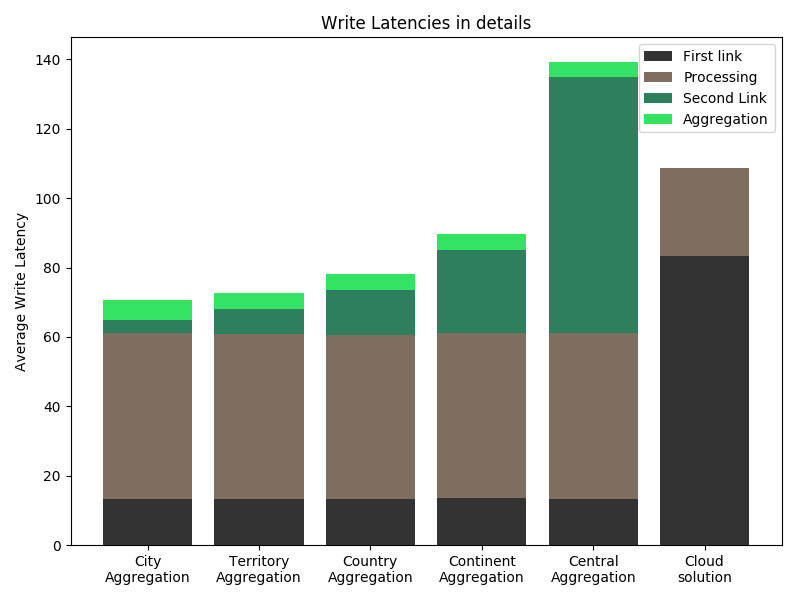
\includegraphics[width=0.95\linewidth]{Figures/Evaluation/write-by-latency2.png}
    \caption{Details on the average write latency compared between various aggregation in the edge setup and compared to the cloud setup.}
    \label{fig:write-by-latency2}
\end{figure}

In Figure \ref{fig:write-by-latency2} we can see the average write latency for each setup. For the edge approach we show the result of five different setups with five different levels of aggregation (city, territory, country, continent, central).
This average write latency comes from four different operations:
\begin{itemize}
    \item First link latency: latency of the communication between the client and the receiving machine.
    \item Processing latency: latency that considers the wait time for a core to be free and the processing time for the data sent by the client. We can see in the plot that the processing time of the cloud solution is close to half of the processing time in the edge setups, this is due the fact that the core bandwidth of a core in \inlinecode{ProcessingLocationCentral} is supposed to be double the core bandwidth of a core in \inlinecode{ProcessingLocationDistrict}.
    \item Second link latency: latency of the communication between the receiving  \inlinecode{ProcessingUnit} and the aggregating \inlinecode{ProcessingUnit}. This latency is only present in the setups using the edge approach.
    \item Aggregation latency: time required by the aggregating \inlinecode{ProcessingUnit} to save the data received from the \inlinecode{ProcessingLocationDistrict}. This time is the sum of the wait time for a core to be free and the time to save the processed data.
\end{itemize}

This result shows that with the edge approach using any aggregation level we have a smaller average latency than the cloud solution thanks to a much smaller travel distance needed to reach the aggregating \inlinecode{ProcessingUnit}. The only exception is the central aggregation of the edge approach, which is expected since it has the same travel distance of the cloud solution, but by doing the processing on the lower level of the hierarchy we have a smaller processing power.

Using this same experiment we now analyze the huge improvements our edge approach gives to the traffic in the network.

\begin{figure}[H]
    \centering
    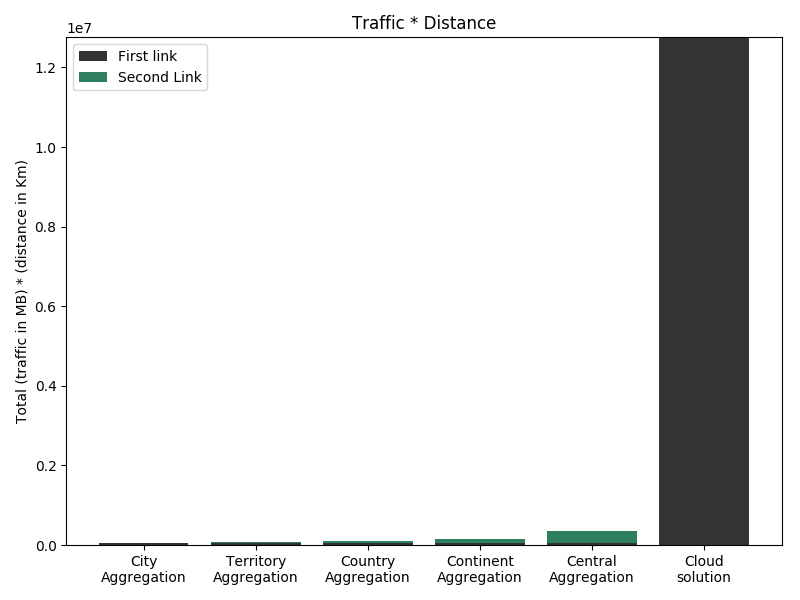
\includegraphics[width=0.95\linewidth]{Figures/Evaluation/write-by-traffic1.png}
    \caption{Traffic per distance generated in the network.}
    \label{fig:write-by-traffic1}
\end{figure}

In Figure \ref{fig:write-by-traffic1} we show the total traffic in megabytes multiplied by the distance travelled. This visualization is used to show that the cloud solution clogs the entire network, instead by processing the data near the client we obtain a huge saving in terms of bandwidth used in the network.

\begin{figure}[H]
    \centering
    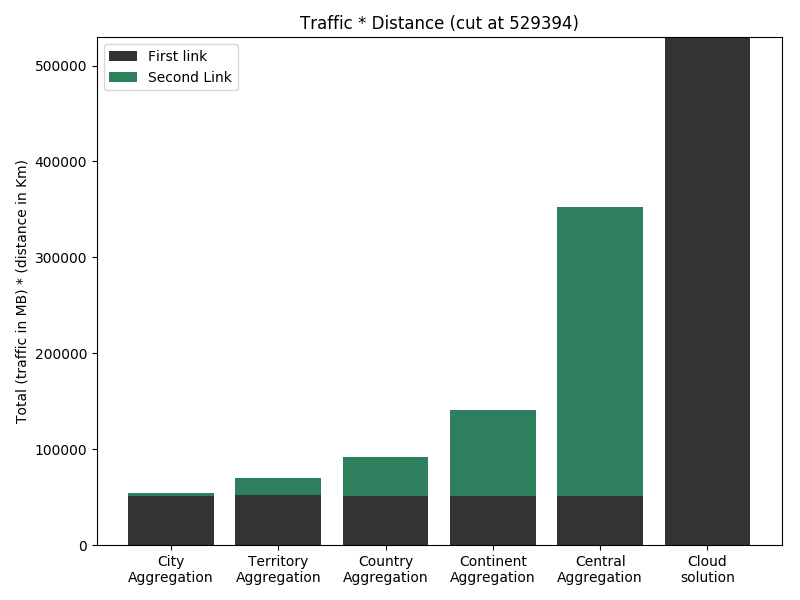
\includegraphics[width=0.95\linewidth]{Figures/Evaluation/write-by-traffic2.png}
    \caption{Traffic per distance generated in the network (cut at a lower traffic*distance value).}
    \label{fig:write-by-traffic2}
\end{figure}

In Figure \ref{fig:write-by-traffic2} we zoom on the values of the setups of the edge approach by cutting the plot at a lower traffic*distance value. We can see how the traffic*distance values in the first link for the edge approach are very much similar since in all five setups we have the same communication between the \inlinecode{DataProducerClient} and the \inlinecode{ProcessingLocationDistrict}. While for the second link we find an increase in the traffic*distance due to the fact that the distance increases between the \inlinecode{ProcessingLocationDistrict} and the aggregating \inlinecode{ProcessingUnit}.


\subsubsection{Write all levels}
In this experiment, for the edge approach, we suppose that the developer uses the boolean \inlinecode{saveAlsoInIntermediateLevels} set to \inlinecode{true} and sets the \inlinecode{referringAreaType} in our framework to the highest level of the hierarchy (central). Meaning that all writes made at the receiving  \inlinecode{ProcessingLocationDistrict} are forwarded to the upper levels. This setup is compared to the cloud setup in which data are sent to a central data center that can aggregate them by location.

Writes to upper levels happen in parallel, so we expect to have an average latency similar to the latency of the edge setup with central aggregation of the previous experiment. This is in fact what we obtain as can be seen in Figure \ref{fig:write-all-latency}. In terms of latency we are clearly in a case of disadvantage here since as it has been seen in the previous experiment that by doing a central aggregation, like the cloud approach does, we are not exploiting our edge approach to the max.

\begin{figure}[H]
    \centering
    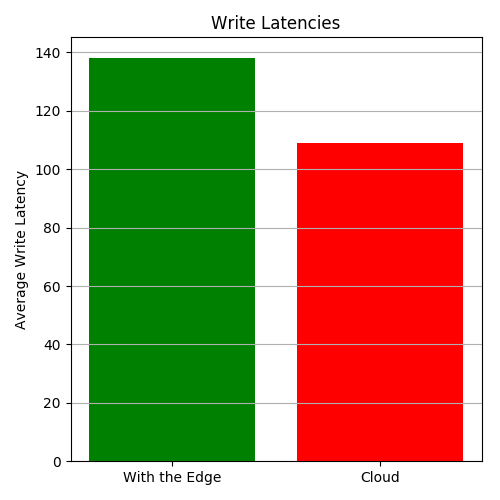
\includegraphics[width=0.75\linewidth]{Figures/Evaluation/write-all-latency.png}
    \caption{Average write latency of the single edge setup compared to the cloud setup.}
    \label{fig:write-all-latency}
\end{figure}

Many more messages are sent in parallel to the various aggregating \inlinecode{ProcessingUnit} so we expect the traffic*distance in the network to increase compared to the previous experiment. This is in fact true as can be seen in Figure \ref{fig:write-all-traffic1}, but still the cloud setup clogs the network 2000\% more than the edge setup.

\begin{figure}[H]
    \centering
    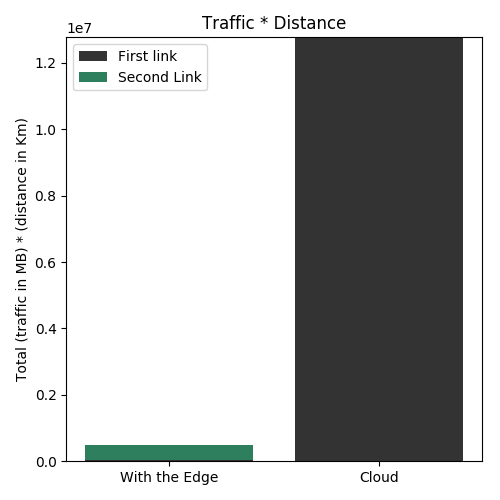
\includegraphics[width=0.75\linewidth]{Figures/Evaluation/write-all-traffic1.png}
    \caption{Traffic per distance generated in the network.}
    \label{fig:write-all-traffic1}
\end{figure}

We saw in this experiment that even in a disadvantage situation where our approach is used to aggregate the data in a central manner, which is not the intended use case, the increase in write latency is less than 27\%, but the improvement in terms of traffic sent in the network is tremendous.


\subsubsection{Write all levels, with CPU core performance as parameter}
As in the previous experiment we are working in a scenario where the developer imposes writes on all levels in the edge approach.

In our simulation we represented the performance of the cores as a processing bandwidth, so we specified how much data a core can process in a second. In the previous experiments we used the default values reported in Section \ref{section:simulation_setting}, so we arbitrarily assumed that the \inlinecode{ProcessingLocationDistrict} and \inlinecode{ProcessingLocationCity} have 50\% of the performance of \inlinecode{ProcessingLocationCentral}. We now analyze the behaviour of the latency while slowly changing this percentage to show that the increase in write latency is not substantial.

\begin{figure}[H]
    \centering
    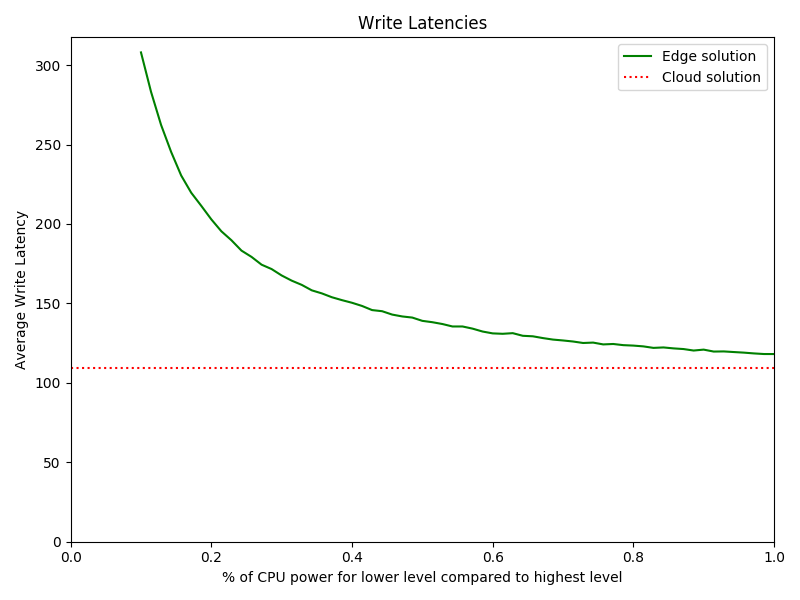
\includegraphics[width=0.95\linewidth]{Figures/Evaluation/write-all-cpu-latency.png}
    \caption{Average write latency of the edge solution while changing the CPU core performance of lower levels}
    \label{fig:/write-all-cpu-latency}
\end{figure}

In Figure \ref{fig:/write-all-cpu-latency} it is shown the changing write latency of the edge solution due to the changing performance of the \inlinecode{ProcessingUnits} cores, compared to the constant latency of the cloud solution. From 1.0 to 0.40 we have an almost linear increase, which is not substantial. Then down from 0.40 the cores can't keep up with the requests and start to put them in queue, creating an exponential increase in the latency.

So this experiment shows the following:
\begin{itemize}
    \item By having a lower performance in the \inlinecode{ProcessingUnits} at the edge the processing latency increase linearly, making the write latency also increase linearly;
    \item By having a lower performance in the \inlinecode{ProcessingUnits} at the edge it becomes easier to reach a limit where the cores can't keep up with the requests, creating an exponential increase in the write latency.
\end{itemize}















\iffalse
This chapter shows the results of the experiments carried out to assess your contribution, usually compared to state of the art solutions. In the proposed structure, we separate experiments setup from experiment results, in which we list the experiments. This is especially convenient in case the setting is the same or very similar for all the experiments. Should this not be the case, you may consider instead to structure each experiment is a section/subsection and embed both setting and result inside it.

\begin{example}
In this chapter, we present experimental results on the algorithms proposed and we compare them with state of the art methods.
\end{example}

\section{Experimental setting}

First, describe the experimental setting. The setting usually contains:
\begin{itemize}
\item the dataset(s) used for the experiments;
\item the baselines, namely the other solutions with which you are comparing yours.
\end{itemize}

\begin{example}

\begin{table}[H]
\centering
\renewcommand{\arraystretch}{1.2}
\begin{tabular}{|l|c|c|c|c|c|}\hline
\textbf{Name}&$n$&$m$\\ \hline\hline
Email&1005&25571\\ \hline
\end{tabular}
\caption{Dataset used for the experiment.}
\label{tb:elf_datasets}
\end{table}

\paragraph{Datasets} \autoref{tb:elf_datasets} shows the characteristics of the real-world dataset used for the experiment. The dataset, provided by SNAP \cite{snapnets}, \emph{email-Eu-core}, has been generated using email data from a large European research institution. A directed edge $(u, v)$ means that person $u$ sent an e-mail to person $v$.

As widely done in literature, we assigned the ground-truth influence probabilities according to the weighted cascade model, that is, $p_{u,v}=\frac{1}{|In(v)|}$, for each edge $(u,v) \in E$.

\paragraph{Algorithms}

For the learning process, we use the Thompson Sampling (TS) as principal exploration strategy (\autoref{alg:cts}). For the sake of completeness, we show also results with a Pure Exploitation (PE) approach, in which the oracle is fed with the mean estimates of the influence probabilities at each round.

\end{example}

\section{Results}

In this section, we show and comment the results obtained from the experiments. Remember to comment every result and every figure you decide to insert in the thesis.

\begin{example}
\paragraph{Experiment 1}

\begin{figure}[H]
  \centering
  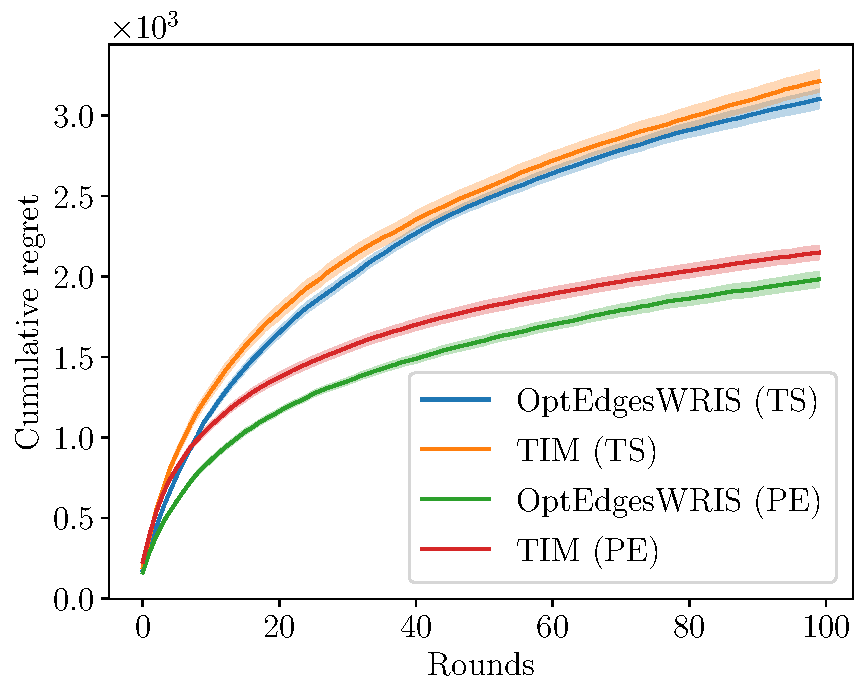
\includegraphics[width=.65\textwidth]{experiments/regret.pdf}
\caption{Cumulative regret in Email-In4 with 95\% confidence interval.}
\label{fig:exp_email}
\end{figure}

In this experiment, we test the algorithms on Email over a time horizon of $T=100$ rounds. The objective is to show the performances of the algorithms. The results have been averaged over 30 runs. \autoref{fig:exp_email} shows the cumulative regret, with a 95\% confidence interval.

As shown in the plot, our algorithm performs better with both the exploration strategies. However, the gain on TIM is more evident with the PE strategy, specially in the first rounds.
\end{example}
\fi

\chapter{Conclusions and future developments}
\label{ch:conclusions}

In this chapter, you present the conclusions of your thesis and a couple of possible future works to extend your results. First of all, you should briefly repeat the problem you addressed in the thesis. Then, you report your achievements and how they improve the state of the art.

\section{Conclusions}
In this thesis, we analyzed the problem of ... . We proposed a new approach that ... . We tested this method on ... . Reported results show that our proposal outperforms the state of the art method.

\section{Future works}
There are several appealing paths for future works. A possible extension could be to ... .


%-------------------------------------------------------------------------
%	BIBLIOGRAPHY
%-------------------------------------------------------------------------

\addtocontents{toc}{\vspace{2em}} % Add a gap in the Contents, for aesthetics
\bibliography{Thesis_bibliography} % The references information are stored in the file named "Thesis_bibliography.bib"

%-------------------------------------------------------------------------
%	APPENDICES
%-------------------------------------------------------------------------

\cleardoublepage
\addtocontents{toc}{\vspace{2em}} % Add a gap in the Contents, for aesthetics
\appendix
\chapter{Appendix}

The resulting artifacts of our research have been released as open-source software \cite{thesis-github}. Here we present a concise guide on how to run and use these artifacts.

Note that this guide is not meant to be universal, and instead shows the steps we performed to run the system in our specific setup.

\section{Running the Prototype}
For running the prototype we used the \textit{faas} flavour of \textit{OpenFaas}, which runs on top of \textit{Kubernetes}. If \textit{faasd}, the lighter version of \textit{OpenFaas}, is needed, then a slightly different setup would be necessary.


\subsection{Prerequisites}
The following applications and Command Line Interface programs are needed to setup the framework:
\begin{itemize}
    \item \textbf{arkade}: \textit{arkade} provides a portable marketplace for downloading popular devops CLIs and installing helm charts;
    \\It can be installed with \inlinecode{curl -sLS https://get.arkade.dev | sudo sh};
    \\More info at this link \href{https://github.com/alexellis/arkade}{github.com/alexellis/arkade}
    
    \item \textbf{faas-cli}: the Command Line Interface of \textit{OpenFaas};
    \\It can be installed with \inlinecode{arkade get faas-cli};
    
    \item \textbf{helm}: the \textit{Kubernetes} package manager;
    \\It can be installed with \inlinecode{arkade get helm};
    
    \item \textbf{minikube}: a local \textit{Kubernetes} engine;
    \\On our setup running macOS Big Sur with a x86-64 CPU it was installed with \inlinecode{brew install minikube};
    \\More info at this link \href{https://minikube.sigs.k8s.io/docs/start/}{minikube.sigs.k8s.io/docs/start/}
\end{itemize}


\subsection{Kubernetes Setup}
To run \textit{Kubernetes} we used \textit{minikube}, a software which allows to easily create a Virtual Machine environment equipped with \textit{Kubernetes}. Note that in a production environment \textit{minikube} is not recommended, but in our emulation it was perfect to run multiple nodes that emulate the nodes in an edge network.

The following are the commands we used to start the Virtual Machines (note that as virtualization software connected to \textit{minikube} we used \textit{Parallels Desktop}):
\begin{lstlisting}[language=bash]
minikube delete --all  # Delete previous VMs

minikube config set driver parallels  # Set Parallels as virtualization software

minikube config set cpus 2  # Set 2 CPUs per VM

minikube config set memory 2048  # Set 2048MB of RAM per VM

minikube start --profile p1  # Start a new VM with name p1

minikube start --profile p2  # Start a new VM with name p2

minikube ip --profile p1  #  Get IP address of p1

minikube ip --profile p2  #  Get IP address of p2

kubectl config get-contexts  #  Print Kubernetes contexts (should show two Kubernetes machines, p1 and p2)

kubectl config use-context p1  #  Use p1 for the next commands

kubectl get po -A  # List all pods running on Kubernetes
\end{lstlisting}

At the end of these commands the results are, in this case, the creation of two empty VMs running \textit{Kubernetes}, without any external software installed on it.
Now the goal is to install the framework we developed on top of these \textit{Kubernetes} installations.

Three steps are still needed:
\begin{itemize}
    \item Install the \textit{faas} flavour of \textit{OpenFaas} on top of \textit{Kubernetes};
    \item Install \textit{Redis} on top of Kubernetes;
    \item Deploy on \textit{OpenFaas} the function we developed that allows locations to receive forwarded write actions.
\end{itemize}


\subsection{OpenFaas Setup}
On each \textit{Kubernetes} environment it is needed to install \textit{OpenFaas}. The installation can be performed in the following way:
\begin{lstlisting}[language=bash]
# Use p1 for the next commands (should be changed for every VM)
kubectl config use-context p1

# Apply OpenFaas configuration
kubectl apply -f https://raw.githubusercontent.com/openfaas/faas-netes/master/namespaces.yml

# Write OpenFaas password in a secret
kubectl -n openfaas create secret generic basic-auth --from-literal=basic-auth-user=admin --from-literal=basic-auth-password="customOpenFaasPassword"  

# Install OpenFaas
helm upgrade openfaas --install openfaas/openfaas --namespace openfaas --set functionNamespace=openfaas-fn --set basic_auth=true

# Install the cron addon
helm upgrade --install cron-connector openfaas/cron-connector --namespace openfaas

# Login to OpenFaas running on machine p1 that we have just installed
echo "customOpenFaasPassword" | faas-cli login -u admin --password-stdin --gateway http://$(minikube ip --profile p1):31112
\end{lstlisting}
At the end of this step we have the \textit{faas} flavour of \textit{OpenFaas} installed on every node.


\subsection{Redis Setup}
On each \textit{Kubernetes} environment it is needed to install \textit{Redis}. The installation can be performed in the following way:
\begin{lstlisting}[language=bash]
# Use p1 for the next commands (should be changed for every VM)
kubectl config use-context p1

# Install Redis
helm install my-openfaas-redis bitnami/redis --namespace openfaas-fn --set auth.password="customRedisPassword" --set master.persistence.enabled=false
\end{lstlisting}
At the end of this step we have a Redis instance installed on every node on top of \textit{Kubernetes}.
Now we can put all the IP addresses of the machines in the JSON of the infrastructure.
\\The IP addresses can be obtained, as seen, with \inlinecode{minikube ip --profile p1}.


\subsection{The Receiver Function}
After the infrastructure JSON file is ready we can deploy the function "edge-db-data-receiver" which allows locations to receive forwarded write actions.
\begin{lstlisting}[language=bash]
# Move in the directory where the "edge-db-data-receiver" function is stored
cd ./framework/functions-main/

# Build and publish the "edge-db-data-receiver" function on a Docker Registry
faas-cli publish --filter edge-db-data-receiver --platforms linux/arm/v7,linux/amd64

# Deploy the function on every level, except the lowest level
deployer deploy edge-db-data-receiver infrastructure.json --inEvery city
deployer deploy edge-db-data-receiver infrastructure.json --inEvery country
deployer deploy edge-db-data-receiver infrastructure.json --inEvery continent
\end{lstlisting}
At the end of this step the framework is ready to receive custom functions, that can be created by the developer as seen in Chapter \ref{ch:prototype}. 


\subsection{Deploying Custom Function}
To deploy new custom functions it is simply needed to perform the following commands:
\begin{lstlisting}[language=bash]
# Move in the directory where the "stack.yml" file is defined
cd ./framework/functions-main/

# Build and publish the function on a Docker Registry
faas-cli publish --filter my-function-name --platforms linux/arm/v7,linux/amd64

# Deploy the function
deployer deploy my-function-name infrastructure.json --inEvery district --inAreas italy paris --exceptIn milan
\end{lstlisting}


\section{Debugging the Prototype}

\subsection{Debugging Custom Functions}
The following commands can be used to print the logs of a function:
\begin{lstlisting}[language=bash]
# Select which node to debug
kubectl config use-context p1

# Print the logs of the function running on that node
kubectl logs -n openfaas-fn deploy/my-function-name -f
\end{lstlisting}
Or alternatively the \textit{faas-cli} can be used as follows:
\begin{lstlisting}[language=bash]
faas-cli logs my-function-name --gateway http://$(minikube ip --profile p1):31112
\end{lstlisting}


\subsection{Debugging the Framework}
To debug the framework itself or to understand why a function is having issues starting up, the following commands can be used:
\begin{lstlisting}[language=bash]
# Select which node to debug
kubectl config use-context p1

# List all pods and components running on Kubernetes
kubectl get po -A

# Print many info about a single component (in this example the gateway component)
kubectl describe -n openfaas deploy/gateway
kubectl logs -n openfaas deploy/gateway

# Print events happened in the openfaas namespace
kubectl get events -n openfaas --sort-by=.metadata.creationTimestamp
\end{lstlisting}


\section{Running the Simulation}
The Simulation is composed of many Phython files, one file for each scenario. To run a scenario it is simply possible to run the Python file with a Python IDE (e.g., PyCharm).

Note that a single configuration in some scenarios may simulate millions of machines and the simulation of such a huge number of machines requires an high utilization of RAM.
For example the scenario included in \inlinecode{simulation\_read\_district\_level\_clients\_ratio.py} can use up to 14 GB or RAM for the simulation.
If such usage of RAM becomes a problem, it is possible to make a modification to the trade-off between the speed of the execution of the simulation and the usage of RAM by modifying the following line:\\
\inlinecode{pool = multiprocessing.Pool(processes=4)}\\
and replacing the 4 with a lower number to use less RAM, while also using less parallelism for the simulation, resulting in a slower execution. In practice this number represents how many configurations of the scenario can be run in parallel on the given processes.



\chapter{Running the Simulation}
TODO


% LIST OF FIGURES
\listoffigures

% LIST OF TABLES
\listoftables

% LIST OF SYMBOLS
\chapter*{List of Acronyms and Abbrevations}
\begin{table}[H]
\begin{tabular}{p{2cm}l}
API    & Application Programming Interface                         \\[5pt]
BGP    & Border Gateway Protocol                                   \\[5pt]
CDN    & Content Delivery Network                                  \\[5pt]
CLI    & Command Line Interface                                    \\[5pt]
FaaS   & Function-as-a-Service                                     \\[5pt]
GB     & Gigabyte                                                  \\[5pt]
GPS    & Global Positioning System                                 \\[5pt]
HTTP   & HyperText Transfer Protocol                               \\[5pt]
ICFEC  & IEEE International Conference on Fog and Edge Computing   \\[5pt]
ID     & Identifier                                                \\[5pt]
IDE    & Integrated Development Environment                        \\[5pt]
IP     & Internet Protocol                                         \\[5pt]
IoT    & Internet-of-Things                                        \\[5pt]
JSON   & JavaScript Object Notation                                \\[5pt]
KB     & Kilobyte                                                  \\[5pt]
MB     & Megabyte                                                  \\[5pt]
OS     & Operating System                                          \\[5pt]
RAM    & Random Access Memory                                      \\[5pt]
RQ     & Research Questions                                        \\[5pt]
UI     & User interface                                            \\[5pt]
URL    & Uniform Resource Locator                                  \\[5pt]
VM     & Virtual Machine                                           \\[5pt]
\end{tabular}
\end{table}


% INFORMAL ACKNOWLEDGEMENTS
%\chapter*{Acknowledgments}
TODO


\iffalse
Here you can insert optionally the acknowledgments for who had a significant importance for the accomplishment of this goal. These acknowledgments are less formal than the ones at the beginning of the thesis and are not listed in the table of contents.
\fi


\cleardoublepage

\end{document}
